%\documentclass[aps,prb]{revtex4}
%\documentclass[aps,prb,twocolumn]{revtex4-1}
\documentclass[showpacs,aps,prb,reprint,superscriptaddress]{revtex4-2}
%\documentclass[showpacs,aps,prl,reprint,superscriptaddress,showkeys,floatfix,citeautoscript]{revtex4-1}
\usepackage{bm}
%\usepackage{subfig} % LUIS: This package messes with the captions.
\usepackage{graphicx}
\usepackage{graphics}
\usepackage{amsmath,amssymb,amstext}
\usepackage{amsfonts}

\usepackage{epstopdf}
\usepackage{hyperref}
\hypersetup{
    colorlinks,%
    citecolor=blue,%
    linkcolor=blue,%
    urlcolor=blue
}
%\usepackage{pgf}
\usepackage{tikz}\usetikzlibrary{petri}
%\usepackage{bbold}
%\usepackage{makeidx}
\newcommand{\TS}[1]{{$\rightarrow$ {\sl#1}}}
\newcommand{\LUIS}[1]{\textcolor{blue}{\fbox{Luis} {\sl#1}}}
\newcommand{\Jesus}[1]{\textcolor{red}{\fbox{Jesus} {\sl#1}}}
\newcommand{\change}[1]{\textcolor{red}{\sl#1}}
\begin{document}


\newcommand{\be}   {\begin{equation}}
\newcommand{\ee}   {\end{equation}}
\newcommand{\ba}   {\begin{eqnarray}}
\newcommand{\ea}   {\end{eqnarray}}
\newcommand{\ve}  {\varepsilon}

\newcommand{\nhat}{\hat{n}}
\newcommand{\veck}{\textbf{k}}
\newcommand\ep{\epsilon}
\newcommand\g{\gamma}
\newcommand\s{\sigma}
\newcommand\up{\uparrow}
\newcommand\dw{\downarrow}
\newcommand\down{\downarrow}
\newcommand{\ed}[1]{\ep_{d#1}}
\newcommand{\ket}[1]{\vert #1 \rangle}
\newcommand{\ann}{a^{\dagger}}
\newcommand{\dann}{d^{\dagger}}
\newcommand{\tdots}{t_{dots}}
\newcommand{\gammaA}[1]{\gamma_{A,#1}}
\newcommand{\gammaB}[1]{\gamma_{B,#1}}
\newcommand{\Green}[1]{G_{#1}(\omega) }

\newcommand{\GreenG}[2]{G_{#1}^{ #2} (\omega) }
%\newcommand{\bra}[3]{\langle {#3} \vert}

\newcommand{\super}{\vert \Delta \vert}





%%%%%%%%%%%%%%%%%%%%%%%%%%%%%%%%%%%%%%%%%%%%%%%%%%%%%%%%%%%%%%%%%%%%%%%%%%%%%%%
\title{ Manipulation of Majorana zero-modes using double quantum dots }

\author{Jesus D. Cifuentes}
\affiliation{Instituto de F\'{\i}sica, Universidade de S\~{a}o Paulo,
C.P.\ 66318, 05315--970 S\~{a}o Paulo, SP, Brazil}
\author{Luis G.~G.~V. Dias da Silva}
\affiliation{Instituto de F\'{\i}sica, Universidade de S\~{a}o Paulo,
C.P.\ 66318, 05315--970 S\~{a}o Paulo, SP, Brazil}

\date{ \today }

\begin{abstract}
Majorana zero modes (MZMs) emerging at the edges of topological superconducting wires are a promising platform for fault-tolerant quantum computation. Novel proposals use quantum dots (QDs) coupled to the end of these wires to detect Majorana signatures. This detection method provides the following advantages: 1) It allows to study the prospective coexistence of Kondo-Majorana signatures, which have been recently reported in experiments.  2)  Today's precise experimental control over QDs offers the unique possibility of manipulating  MZMs inside multi-dot systems, which recently enlightened the design of scalable quantum architectures.The simplest case where Majorana manipulation is possible is in a double quantum dot (DQD). This model offers several possibilities for manipulation of MZMs, including different geometric configurations of the dots, from symmetric and ``in-series'' couplings to T-shaped junctions. By comparing exact analytical solutions in the non-interacting system and numerical renormalization-group results for interacting QDs, we were able to characterized the displacements of the MZM in a DQD. 


% In this project we perform analytical (non-interacting) and numerical(interacting) quantum transport studies of the transition of the Majorana signature. By tuning the model parameters we show that it is possible to control the localization of the MZM inside the DQD. 


% Majorana zero modes (MZMs) appearing at the edges of topological superconducting wires are a promising platform for fault-tolerant quantum computation. Novel proposals use MZMs tunneling inside quantum dots (QDs) to implement quantum architectures because today?s precise experimental control over the QD parameters offers the unique possibility of manipulating the Majoranas inside multi-dot systems. The simplest case where Majorana manipulation is possible is in a double quantum dot (DQD). This model shows several possibilities for manipulation of MZM, including different geometric couplings such as linear forms of T-junctions. In this project we perform analytical (non-interacting) and numerical(interacting) quantum transport studies of the transition of the Majorana signature. By tuning the model parameters we show that it is possible to control the localization of the MZM inside the DQD. 




% Majorana fermions appearing at the edges of topological superconducting wires are a promising platform for fault-tolerant quantum computation. Novel proposals use Majorana modes tunneling inside quantum dots (QDs) to implement quantum architectures, because today?s precise experimental control over the QD parameters offers the unique possibility of manipulating the Majorana modes inside multi-dot systems. The simplest case where Majorana manipulation is possible is in a double quantum dot (DQD). So far, no complete analysis of this basic structure has been done. This  project fills this gap by realizing an exact quantum transport study of the effects of coupling a Majorana mode with a DQD. By tuning the model parameters we show that it is possible to control the localization of the Majorana signature in the DQD. 




\end{abstract} 
%\pacs{ APS does not use it anymore}
%\keywords{Quantum Spin-Hall effect, Edge transport, Topological insulators}

\maketitle


%%%%%%%%%%%%%%%%%%%%%%%%%%%%%%%%%%%%%%%%%%%%%%%%%%%%%%%%%%%%%%%%%%%%%%%%%%%%%%%v

%\pacs{ APS does not use it anymore}
%\keywords{Quantum Spin-Hall effect, Edge transport, Topological insulators}

\maketitle


%%%%%%%%%%%%%%%%%%%%%%%%%%%%%%%%%%%%%%%%%%%%%%%%%%%%%%%%%%%%%%%%%%%%%%%%%%%%%%%
\section{Introduction}
\label{sec:Intro}


The pursuit of Majorana quasi-particles in topological superconductors has attracted significant attention in the last decades \cite{alicea_new_2012,beenakker_search_2013}.  Since the first Kitaev's toy models \cite{kitaev_unpaired_2001,kitaev_fault-tolerant_2003} claiming promising applications to quantum computing, the field evolved rapidly towards physical realizations of the Kitaev chain.  The last few decades have been full of excitement as new technological innovations  allowed to document several times the observation of Majorana signatures \citep{mourik_signatures_2012,das_zero-bias_2012,deng_anomalous_2012,nadj-perge_observation_2014,deng_majorana_2016,zhang_quantized_2018}. One of the most promising structures is the so-called Majorana wire, which recipe consists in growing semiconducting wires with strong-orbit-coupling over proximity-induced topological (p-wave) superconductors.  

\change{These Majorana signatures are characterized by the emergence of robust zero modes localized at the edges of the material. Recently, the so-called Majorana zero-modes (MZM) have been found in superposition with other zero-bias phenomena such as the Kondo effect \cite{lee_zero-bias_2012}. This situation has put in question the discovery of Majorana quasi-particles. Therefore, current experimental proposals focus on methods to certify their existence, well by adding external parameters like magnetic fields that could distinguish the  MZMs from the other effects, or by measuring Majorana's unique property of non-abelian statistics \cite{aasen_milestones_2016,sarma_majorana_2015,heck_coulomb-assisted_2012}. Although this last property is fundamental to implement fault-tolerant quantum computers, it has never been measured. In part, because it involves achieving an unprecedented precise control over Majorana quasi-particles.}  



% implementing braiding protocols , a key basic operation for topological quantum computing  that takes advantage of the Majorana's unique property of non-abelian statistics. Nonetheless, braiding are still far since they require Majorana manipulation that have never been measured.  


A promising method to detect MZMs consists in attaching a quantum dot (QD) to the edges of a Majorana chain in the topological phase and executing transport measurements through the QD \cite{liu_detecting_2011}.  In such arrangement, the MZM at the end of the chain leaks inside the QD \cite{vernek_subtle_2014} producing a zero-bias conductance peak of half a quanta $\frac{e^{2}}{2h}$ through the dot. \change{ Recently, experiments including hybrid Majorana-QD systems have been performed confirming the viability of this proposal\cite{deng_majorana_2016} . This method offers several advantages: 1) The qubit information  is not completely destroyed, in contrast to other detection methods such as tunneling spectroscopy. 2) If performed under the  Kondo temperature $T_k$, it allows to observe the MZM co-existing with the Kondo peak \cite{lee_kondo_2013,ruiz-tijerina_interaction_2015,gorski_interplay_2018} , and to study how to distinguish both effects. 3) Today's precise experimental control over the QD parameters offers the unique possibility of manipulating MZMs inside multi-dot systems, hence providing enlightening proposals to measure non-abelian statistics \cite{malciu_braiding_2018} and to design of quantum architectures  \cite{barkeshli_physical_2015,karzig_scalable_2017}. }



%   In addition, the similarity of this phenomenon with the Kondo effect,\cite{hewson_kondo_1997,wilson_renormalization_1975} where the zero-bias conductance peak takes  $\frac{e^{2}}{h}$, motivated the study of combined Kondo-Majorana physics in this system. \cite{lee_kondo_2013,ruiz-tijerina_interaction_2015} This project revealed the existence of a region of parameters where bo


 The simplest case where Majorana manipulation is possible is in a double quantum dot (DQD). Tunneling Majorana modes in these basic structures have inspired theoretical studies \cite{silva_andreev_2016,ivanov_coherent_2017,Loss2019} \Jesus{Added citation} and experimental setups confirming the observations of Andreev molecules \cite{su_andreev_2017}. Even though quantum tunneling of a MZM into a double dot offers several possibilities for manipulation of MZM,  there is still no complete analysis of the transitions of the Majorana signatures between the QDs in this model. 
 
 
 In this paper, we explore the different possibilities for Majorana manipulation in a device consisting of a DQD coupled to a MZM and a metallic lead (See Fig.\ \ref{fig:GenModel}). The simplicity of this model allows us to explore analytically different geometries of QD's from symmetric and ``in-series'' couplings to T-shaped junctions (Fig.\ \ref{fig:MajoranaModels}). We considered both non-interacting and interacting regimes, observing major agreement between both approaches about the location of the Majorana signature.
 
 We performed a detailed study of the non-interacting DQD limit, by using Zubarev's procedure  \cite{zubarev_double-time_1960} to provide an exact formula to calculate the spectral functions. For the interacting case, we resort to numerical renormalization group (NRG)\cite{bulla_numerical_2008} calculations for this model.
 While the non-interacting regime is suitable to obtain exact expressions for the Green function, the interacting case  shows how the Majorana signature co-exists with strongly correlated phenomena such as the Kondo effect \cite{hewson_kondo_1997} and RKKY interactions.   \cite{ruderman_indirect_1954,kasuya_theory_1956,yosida_magnetic_1957} 


This paper is organized as follows. In Sec.\ \ref{sec:modelmethods} we describe the model of a DQD coupled to a MZM and to a metallic lead, as well as the methods used.  The results are presented in section \ref{sec:results} where we compare the non-interacting density of states (LDOS) \ref{subsect:non-int} with the low-energy  interacting results \ref{subsec:Interacting}. Finally, our conclusions are given in Sec.\ \ref{sec:Conclusions}.


  % So far, no complete analysis of this simple case has been done. The goal of this  project is to fill this gap by realizing a full quantum transport study of the effects of coupling a Majorana mode with a double quantum dot.  By tuning the QD gate voltages and the Majorana couplings we will be able to probe the mobility of the Majoranamodes through the dots. 




% \LUIS{In this paper, we ...} 
%   In this paper we  considered both interacting and non-interacting cases. For interacting systems we used a obtained the exact transport description . On non-interacting models we used a NRG approach.   We found that in symmetric couplings  In the non-interacting case, we confirmed that shifting the QD?s gate voltage induces the Majorana to tunnel only to the other dot. In addition, an indirect coupling of the second dot could cause destructive interference with the Majorana signature. In the interacting case,  the NRG simulations confirmed these results and showed that other interacting effects -  Kondo effect and RKKY interactions \cite{ruderman_indirect_1954,kasuya_theory_1956,yosida_magnetic_1957} - could coexist with the Majorana signatures. On the other hand, when only one QD is coupled to the leads and the other Dot is attached to the QD,  the Kondo effect is annihilated due to the destructive interference  generated by extra dot. \cite{dias_da_silva_transmission_2008} Our study includes how the Majorana mode interacts with these two effects.  
 


 % These experiments are performed at very low temperatures where the MZM could coexists with the  Kondo effect \cite{lee_kondo_2013,ruiz-tijerina_interaction_2015}.  


% Despite the positive experimental results, their is still certain skepticism about the existence . The zero mode could be the product of other phenomena  such as the Andreev bound states or even the Kondo effect. 

% Specially in the so called Majorana wires, where observations of zero modes have been documented   
%  To the date, extended experiments have documented the observation, of Majorana zero modes \cite{keylist}


%  Some proposals involve the coupling of quantum dot through superconductivity. 

% to create these materials consists in combining superconducting platform with a with strong-orbit coupling

%  % While some proposal include recreations of Kitaev model using quantum dot chains with superconducting couplings \cite

%  To the date, several experimental proposals have been put forward including InSb superconducting wire 
% {}


%  Majorana bound states appearing at the edges of topological superconductors to topological quantum computing
%  Kitaev's toy models  proposing the promising implementation of 

% the fields has evolved rapidly towards physical realizations of the Kitaev chain. To the date 

% The quasiparticle   is proposed to be one of the most promising approaches to fault tolerant quantum computing. Physical implementations of Kitaev's toy model such as Majorana wires and quantum dot chains 


% The quasi-particle initially proposed by Ettore Majorana 

% Predi

% The Majorana quasiparticle, which in Kitaev's toy model was predicted to appear at the edges of topological superconductors 
% ,
% as the real field solution of the Dirac equation describes a fermion which is its own antiparticle.

%  Though no fundamental particle with these characteristics have been found, 


% To the date no fundamental particle with this characteristic has been found. However, 
% Multiple advances in theoretical  followed by successful experimental have led to the observation of Majorana zero modes localized at the edges of topological superconductors. 
% During the last decade multiple advances in theoretical proposals and led to the detection of Majorana zero modes. 
% However,  theoretical research predicts that Majorana zero modes emerge at the boundary of certain type of topological superconductors. \citet{kitaev_unpaired_2001} 
% The induced topological protection and non-abelian statistics makes Majoranas it a promising candidate for  quantum computation
% To exploit this property a basic braiding  protocol 
% Topological algorithms depend on basic baiding  protocol 
% The Majorana quasiparticle as zero mode 
% The last few decades have been full of excitement as new technological innovations  allowed the observation of Majorana signatures in different topological materials. \citep{mourik_signatures_2012,das_zero-bias_2012,deng_anomalous_2012,zhang_quantized_2018} 


% Despite the positive experimental results, their is still certain skepticism about the existence . The zero mode could be the product of other phenomena  such as the Andreev bound states or even the Kondo effect. 

% Now thworetical proposals concentrate in that could differ the Majoranas from these phenomena and implementing the promising braiding protocol.




% This proposal got huge attention 


% \TS{What's next? Manipulation and braiding !}


% Despite the positive experimental results, their is still certain skepticism about the existence of  Majorana Fermions. One of the reasons  is that some properties of Majorana quasiparticles like the expected non-abelian statistics have not been measure. This property is of especial interest due to its promising applications in topological quantum computing. The braiding protocol based on  Majorana's non-abelian statistics is the key to  fault-tolerant quantum computation. \cite{kitaev_fault-tolerant_2003,sarma_majorana_2015} 

% Experimental proposals for braiding measurements have been  proposed  in one dimensional majorana chains.  The system inspired in the famous Kitaev toy model is a promising example of these topological superconductors.  The chain emulates a spinless p-wave superconducting wire. With the adequate combination of magnetic field,  superconducting gap and Rashba spin-orbit coupling  the wire enters into a topological phase in which zero-mode majorana bound states emerge. 

% This is a Majorana signature which produces half of the expected peak by a regular fermion. 



 
%  The idea of using hybrid quantum dot-Majoranaheteroestructures to implemtent quantum gates has aquired wide interest in the last years.  One of the insights of these structures is the posibility of manipunaling  Majoranas  in multidot systems by shifting the QD gate voltages and Hence the approach is suitable for the implementation of braiding procedures . The simplest system where Majorana manipulation is possible is  a  double quantum dot (DQD) coupled to a Majoranachain. So far, no complete analysis of this simple case has been done. The goal of this  project is to fill this gap by realizing a full quantum transport study of the effects of coupling a Majorana mode with a double quantum dot.
 



% In the last few decades the interest in the so called Majorana fermions has been increasing. The particle proposed by the physicist Ettore Majorana  as the real field solution of the Dirac equation describes a fermion which is its own antiparticle, hence it has no charge nor mass. To the date no fundamental particle with these characteristics has been found. However,  theoretical research predicts that Majorana Fermions emerge as quasi-particles at the boundary of certain topological superconductors. \citet{kitaev_unpaired_2001} Recently, the new technological innovations  allowed the observation of Majorana signatures in different topological materials. \citep{mourik_signatures_2012,das_zero-bias_2012,deng_anomalous_2012,zhang_quantized_2018}

% Despite the positive experimental results, their is still certain skepticism about the existence of  Majorana Fermions. One of the reasons  is that some properties of Majorana quasiparticles like the expected non-abelian statistics have not been measure. This property is of especial interest due to its promising applications in topological quantum computing. The braiding protocol based on  Majorana's non-abelian statistics is the key to  fault-tolerant quantum computation. \cite{kitaev_fault-tolerant_2003,sarma_majorana_2015} 

% % Experimental proposals for braiding measurements have been  proposed  in one dimensional majorana chains.  The system inspired in the famous Kitaev toy model is a promising example of these topological superconductors.  The chain emulates a spinless p-wave superconducting wire. With the adequate combination of magnetic field,  superconducting gap and Rashba spin-orbit coupling  the wire enters into a topological phase in which zero-mode majorana bound states emerge. 

% A promising method to detect Majorana modes consists in attaching a quantum dot (QD) to the edges of a Majorana chain in the topological phase and executing transport measurements through the QD. \cite{liu_detecting_2011}  The Majorana mode at the end of the chain then leaks inside the QD \cite{vernek_subtle_2014} which produces a zero-bias conductance peak of half a quanta $\frac{e^{2}}{2h}$ through the dot. This is a Majorana signature which produces half of the expected peak by a regular fermion.  Recently, experiments including hybrid Majorana-QD systems have been performed. \cite{deng_majorana_2016}  In addition, the similarity of this phenomenon with the Kondo effect,\cite{hewson_kondo_1997,wilson_renormalization_1975} where the zero-bias conductance peak takes  $\frac{e^{2}}{h}$, motivated the study of combined Kondo-Majorana physics in this system. \cite{lee_kondo_2013,ruiz-tijerina_interaction_2015} This project revealed the existance of a region of parameters where both, Kondo and Majorana physics, coexist. 

% This idea has turned on new lights into the design of quantum architectures, \cite{barkeshli_physical_2015,karzig_scalable_2017}  because today?s precise experimental control over the parameters of QDs - energy levels, tunneling couplings, etc. - offers the unique possibility of manipulating the Majorana modes inside multi-dot systems. The simplest case where Majorana manipulation is possible is in a double quantum dot. So far, no complete analysis of this simple case has been done. The goal of this  project is to fill this gap by realizing a full quantum transport study of the effects of coupling a Majorana mode with a double quantum dot.  By tuning the QD gate voltages and the Majorana couplings we will be able to probe the mobility of the Majoranamodes through the dots. 
 
% %  The idea of using hybrid quantum dot-Majoranaheteroestructures to implemtent quantum gates has aquired wide interest in the last years.  One of the insights of these structures is the posibility of manipunaling  Majoranas  in multidot systems by shifting the QD gate voltages and Hence the approach is suitable for the implementation of braiding procedures . The simplest system where Majorana manipulation is possible is  a  double quantum dot (DQD) coupled to a Majoranachain. So far, no complete analysis of this simple case has been done. The goal of this  project is to fill this gap by realizing a full quantum transport study of the effects of coupling a Majorana mode with a double quantum dot.
 
 
%   We  considered both interacting and non-interacting cases. For interacting systems we used a obtained the exact transport description . On non-interacting models we used a NRG approach.   We found that in symmetric couplings  In the non-interacting case, we confirmed that shifting the QD?s gate voltage induces the Majorana to tunnel only to the other dot. In addition, an indirect coupling of the second dot could cause destructive interference with the Majorana signature. In the interacting case,  the NRG simulations confirmed these results and showed that other interacting effects -  Kondo effect and RKKY interactions \cite{ruderman_indirect_1954,kasuya_theory_1956,yosida_magnetic_1957} - could coexist with the Majorana signatures. On the other hand, when only one QD is coupled to the leads and the other Dot is attached to the QD,  the Kondo effect is annihilated due to the destructive interference  generated by extra dot. \cite{dias_da_silva_transmission_2008} Our study includes how the Majorana mode interacts with these two effects.  
 
 
%  When both dots are coupled to the leads the Double Quantum Dot exhibits an antiferromagnetic interaction known as  Ruderman-Kittel-Kasuya-Yosida (RKKY) interaction. On the other hand, when only one QD is coupled to the leads and the other Dot is attached to the QD,  the Kondo effect is annihilated due to the destructive interference  generated by extra dot \cite{dias_da_silva_transmission_2008}. Our study includes how the Majorana mode interacts with these two effects.  



%  One of the insights of this method is that the information of the qubit is not completely destroyed as in other methods like tunneling spectroscopy. 
%  When Majoranas are connected to multidot systems it is possible to manipulate the Majorana mode inside the QDs  by tuning the gate voltage and  tunnel couplings. This fa

%following the prescription by \citet{oreg_helical_2010} and \citet{lutchyn_majorana_2010}.   

% Despite the positive experimental results, the proof One of the most promising aplications of Majorana Fermions is the implementaition of  braiding procedures  which are the key to implement fault-tolerant quantum computers. 
% Most of the experiments have been based on tunneling spectroscopy in junctions between TS and non metallic (NM) leads, where resonances have been observed at zero energy, consistent with the presence of Majorana zero\textendash energy modes. A downside of the tunneling spectroscopy technique  is that it probes not only the end of the Topological Superconductor(TS), but its bulk as well ,
% which completely destroys the qubit information. A less destroying



% In addition, the use of QDs favors the manipulation of the Majorana mode through the shifting of the dot gate voltage and the hopping parameters.

 
 




% Then the Majorana  as proposed by  \citet{liu_detecting_2011} and consists in coupling a quantum dot (QD) to the end of a TS. The analysis performed by Liu of this model revealed a  when the TS is in the topological phase,  which a signature of
% Majorana physics. On 2014, \citet{vernek_subtle_2014} showed that the Majorana Bound State at the end of the TS actually leaks inside the QD , which produces the conductance decay. and the model has been based for braiding experimental proposal
% To the date experimental procedures have been put forward. ery recently the first evidence of Majorana end states
% in TS has been found in multiple experiments


% as quasi-particles in certain types of topological materials have increased. The Majoranas are fermions that are their own anti-particle, hence have no charge nor mass. 
% The Majorana is predicted to be one of the most suitable alternatives to implement fault-tolerant quantum computers. Many experiments showing Majorana signatures in the conductivity have been performed. 
% Basics of Majorana Bound states:  zero-energy edge states in 1D topological superconductors.  

% Discovery on semiconductor nanowires \cite{Oreg:Phys.Rev.Lett.:177002:2010,Lutchyn:Phys.Rev.Lett.:77001:2010,Alicea:Reports:2012} etc. Experimental results \cite{Mourik:Science:1003:2012} \LUIS{Add others.}


% Leaking of Majorana to a QD: \cite{vernek_subtle_2014}, Interplay of Kondo and Majorana\cite{ruiz-tijerina_interaction_2015} Important results: Majorana and Kondo co-exist in the quantum dot even if the dot is non-topological.

% More recent experimental results: Deng et al. \cite{deng_majorana_2016} attached a QD to the end of a nanowire.

% Here we study the coupling of a MBS to a \emph{double} quantum dot system. 

% \TS{Punchline} Multidot systems offer the possiblity of ``moving'' Majoranas aroung using gate voltages and couplings. ossibility of Majorana braiding. Here, we study the simplest case, which is a double dot system.

%%%%%%%%%%%%%%%%%%%%%%%%%%%%%%%%%%%%%%%%%%%%%%%%%%%%%%%%%%%%%%%%%%%%%%%%%%%%%%%
\section{Model and methods}
\label{sec:modelmethods}


We consider the setup shown in Figure \ref{fig:GenModel}, in which a single MZM $\gamma_1$ located at the edge of a 1D topological superconductor is coupled to a double quantum dot (DQD) attached to a single metallic lead. The Hamiltonian of the entire system can be expressed as:
%
\begin{equation}
H=H_{\rm DQD}+H_{\rm lead}+H_{\rm DQD-lead}+H_{\rm M-DQD} 
\label{eq:Model}
\end{equation}
%
where the different terms describe, respectively, the (interacting) DQD, the (non-interacting) metallic lead, and the DQD-lead and DQD-MZM couplings:
%The interacting Anderson Model describes the DQD-lead system  
%d_{i\sigma}^{\dagger}d_{i\sigma}
\begin{align}
%\begin{split}
    H_{\rm DQD} =& \!  \sum_{\substack{i\!=\! 1,2 \\ \sigma \!=\! \dw , \up }} \left(\epsilon_{i}+\frac{U_i}{2}\right)\hat{n}_{i\sigma} + \frac{U_i}{2}\left(\sum_{\sigma} \hat{n}_{i\sigma}-1\right)^{2} \nonumber \\ 
& + \sum_{\sigma} \tdots(\dann_{1\sigma}  d_{2\sigma}+\dann_{2\sigma}  d_{1\sigma}) \; ,   \nonumber  \\ 
H_{\rm lead} =&  \sum_{\mathbf{k}\sigma }\epsilon_{\mathbf{k}}c_{\mathbf{k}\sigma}^{\dagger}c_{\mathbf{k}\sigma }  \; ,   \nonumber \\ 
H_{\rm DQD-lead} =&  \sum_{\mathbf{k}\sigma }\sum_{i\!=\!1,2 }V_{i\textbf{k}} c_{\mathbf{k}\sigma }^{\dagger}d_{i\sigma}+V^*_{i\textbf{k}} d_{i\sigma}^{\dagger}c_{\mathbf{k}\sigma } \; ,  \nonumber  \\ 
H_{\rm M-DQD} =&  \sum_{i=1}^2t_{i} \left(d_{i\downarrow}^{\dagger}\gamma_{1}+\gamma_{1}d_{i\downarrow}\right) \; .
%
\label{eq:H_DQD} 
\end{align}
%
In the equations above, $\epsilon_{i}$ is the energy level of dot $i$, $U_i$ is the Coulomb repulsion and $\tdots$ is the coupling parameter between both QDs. The operator $\dann_{i\sigma}$ creates a particle in dot $i$ with spin $\sigma$ and $\hat{n}_{i\sigma}:=d_{i\sigma}^{\dagger}d_{i\sigma}$ is the particle number operator of state $i$.  $c_{\mathbf{k}\sigma }^{\dagger}$ is the creation operator a particle with momentum $\mathbf{k}$ and spin
$\sigma$ in the lead.  $\epsilon_{\mathbf{k}l}$ is the corresponding energy
 and $V_i(\textbf{k})$ describes the tunneling coupling between the lead and dot $i$ . 
%-----------F I G U R E  1 ------
\begin{figure}[t]
\begin{center}
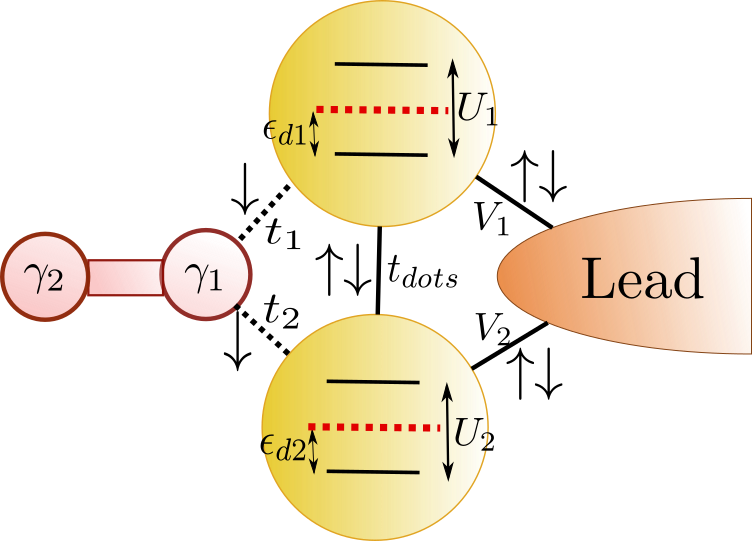
\includegraphics[scale=0.4]{Graficos/GenModel.png}
\end{center}
\caption{ Model for the DQD-Majorana system. Solid lines: Hopping interactions ($t_{dots}$: inter-dot coupling , $V_1,V_2$ couplings of QD1 and QD2 with the lead. ). Dashed lines: Majorana spin-$\dw$ effective couplings \eqref{eq:H_MDQD} $t_1,t_2$. The atomic energy levels appear inside each QD $\ep_1, \ep_2$ are tuned by the gate voltages. The coulomb interaction is represented by $U_1,U_2$.  The red dashed horizontal lines represent the Fermi level.
}
%
\label{fig:GenModel}
\end{figure}
%-----------E N D  F I G U R E  1 ------
% To model the interaction between the DQD and the Majorana Mode we define the Majorana operators as the

It is sometimes useful to recast the last term in Eq.\ (\ref{eq:Model}) in terms of (Dirac) fermionic operators. Following Refs. \onlinecite{lee_kondo_2013,ruiz-tijerina_interaction_2015}, we choose to write the Majorana zero modes $\gamma_1$ and $\gamma_2$ as a superposition of the creation ($f^{\dagger}_\dw$) and annihilation ($f^{ }_\dw$) operators of a spin $\dw$ fermion:
%
\begin{equation}
    \gamma_1 := \frac{1}{\sqrt{2}} \left( f^\dagger_{\dw} + f_{\dw}\ \right) \; , \gamma_2 := \frac{i}{\sqrt{2}} \left( f^\dagger_{\dw} - f_{\dw} \right) \; . \label{eq:MajOp}
\end{equation}


In this representation, the effective coupling between the MZM $\gamma_1$ and the DQD becomes:
%by attaching $\gamma_1$ with the spin-$\dw$ channel in the DQD:

%H_{TS} & = & 2\epsilon_{m}\gamma_{1}\gamma_{2}\nonumber \\
\begin{eqnarray}
    H_{\rm M-DQD} & = &  
    %\sum_{i=1}^2t_{i} %\left(d_{i\downarrow}^{\dagger}\gamma_{1}+\gamma_{1}d_{i\downarrow}\right) + %\epsilon_M \gamma_1\gamma_2. 
    % \\
\sum_{i}t_{i} \left(d_{i\downarrow}^{\dagger}f^\dagger_{\dw} + 
     f_{\downarrow}d_{i\dw} +d_{i\downarrow}^{\dagger}f_{\dw}+
     f_{\downarrow}^{\dagger} d_{i\downarrow}\right) \; , 
    \label{eq:H_MDQD}
\end{eqnarray}
where $t_i$ is the coupling parameter between the Majorana mode and QD $i$. %$\epsilon_m$ is the coupling energy between both Majorana modes.

%in the Majorana-DQD model of Eq. (\ref{eq:Model})

For the purposes of identifying the presence/absence of MZMs ``leaking'' from the edge of the TS into the dots \cite{liu_detecting_2011,vernek_subtle_2014,ruiz-tijerina_interaction_2015}, the quantities of interest are the spin-resolved spectral functions (or, equivalently, the local density of states) of the quantum dots. As usual, the spectral function for spin $\sigma$ in dot $i$ is defined as:
%
%
\begin{equation}
    \rho_{i \sigma}(\omega)\equiv-\frac{1}{\pi} \textrm{Im} \left[G_{d_{i \sigma},d_{i \sigma}^\dagger}(\omega)\right].
    \label{eq:SpecFunc}
\end{equation}
%
where $G_{d_{i \sigma},d_{i \sigma}^\dagger}(\omega) \equiv \langle\langle d_{i \sigma},d_{i \sigma}^{\dagger} \rangle \rangle_\omega$ is the retarded (diagonal) Green's function involving dot $i$ operators $d_{i \sigma}$ and $d_{i \sigma}^\dagger$. Next, we describe the procedures for calculating  $\rho_{i \sigma}(\omega)$ in the regimes of weak ($U_i \ll V$) and strong ($U_i \! \gg\! V$) electron-electron interaction in the dots.


% ----------------------------------------------------------------------------------------------------------
 % ----------------------------------METHODS------------------------------------------------------------------
% --------------------------------------------------------------------------------------------------------------
% \newpage

\subsection{Non-interacting limit: Equations of motion }
\label{sec:non-interactingMethods}

In the non-interacting limit ($U_i\!=\!0$), \change{where $H$ is a quadratic Hamiltonian,} we can obtain analytic expressions for the spectral densities defined in Eq.\ (\ref{eq:SpecFunc}). Using Zubarev's equation of motion (EOM) approach \cite{zubarev_double-time_1960}, we can derive  exact expressions for the Green functions associated to both quantum dot operators $(\Green{d_1d^\dagger_1},\Green{d_2d^\dagger_2})$. 

 The EOM  equations define a $8 \times 8$ linear system where the Hamiltonian parameters $(t_1,t_2,\epsilon_1 \ldots)$ and the energy $\omega$ are taken as algebraic variables. The solution for these types of equations is a \change{finite continued fraction of multivariate polynomials with maximum degree $8$}, which makes it difficult to provide an exact solution using either analytic or numerical methods. To bypass this problem, we introduced a Graph-Gauss-Jordan elimination process \cite{spielman_algorithms_2010} to iteratively solve the coupled equations of motion. We briefly describe the procedure here. 

We begin by representing the Majorana-DQD quantum dot system in a ``flow graph'', where each spin-resolved fermion operator (e.g. $d^{\dagger}_{1 \dw}$, $d_{1 \dw}$, $f_{\dw}$, $f^{\dagger}_{\dw}$, etc.) is represented as a ``vertex". \change{ The coefficients of quadratic terms (such as $d^{\dagger}_{1 \dw} d_{1 \dw}$ or $c^{\dagger}_{k \dw} c_{k\dw}$, etc.) are associated to each node as ``self-energies'' while the coupling terms involving two fermion operators  (such as $d^{\dagger}_{1 \dw} f_{\dw}$ or $d^{\dagger}_{1 \dw} f^{\dagger}_{\dw}$, etc.) are linked to the ``edges" connecting the respective vertexes (see Fig.\ \ref{fig:GaussJordanGraph}). We then proceed to iteratively removing vertexes and edges by rewriting the self-energies and couplings in terms of the eliminated variables, such that each vertex elimination depicts another step in the  Gauss-Jordan process. In the end, the self-energy of the only remaining vertex will contain enough information to compute the target Green function.} 

% We begin by representing the Majorana-DQD quantum dot system in a ``flow graph'', where each spin-resolved fermionic operator (e.g. $d^{\dagger}_{1 \dw}$, $d_{1 \dw}$, $f_{\dw}$, $f^{\dagger}_{\dw}$, etc.) is represented as a ``vertex" while the coupling terms involving two fermionic operators  (such as $d^{\dagger}_{1 \dw} f_{\dw}$ or $d^{\dagger}_{1 \dw} f^{\dagger}_{\dw}$, etc.) are represented as ``lines" connecting the respective vertices (see Fig.\ \ref{fig:GaussJordanGraph}). We then proceed to iteratively eliminating vertices and lines by rewriting the ``target" Green's functions in terms of self-energies and other target GFs. % In the end, we are left with a linear system for the target Green's functions, which can be directly solved.  

This method proved to be efficient in solving complex systems of coupled Green's functions, \change{since the graph elimination process provides a natural linear algorithm to compute the target continued fraction. Moreover, the graphic representation simplifies error correction and allows to identify minimal coupling points, which could reduce the complexity of the solution.} A detailed description is given in Appendix \ref{sec:Appendix_alg}. 

% This method proved to be efficient in solving complex systems of coupled Green's functions. since the graph structure allows us to identify minimum cutting points  and  to compute a recursive formula for the Green function. A more detailed description is given in Appendix \ref{sec:Appendix_alg}.
\LUIS{We need to define what exactly is `` an algorithmic representation of the Green function." } \Jesus{Solved}

% This idea also brings new perspectives to the theory of Majorana systems since the Majorana fermion is an articulation point in the graph that communicates creation and annihilation operators


After applying the Graph-Gauss-Jordan process, we obtain a closed form for the non-interacting Green's functions. For instance the GF for dot 1 (which is directly coupled to the MZM) will be given by:
%
\begin{equation}
G_{{d_{1\downarrow},d_{1\downarrow}^{\dagger}}}\left(\omega\right)=\frac{1}{\omega-\epsilon_{DQD}^{+}-\frac{\left\Vert T_{+}\right\Vert ^{2}}{\omega-\epsilon_{M}-\frac{\left\Vert T_{-}\right\Vert ^{2}}{\omega -\epsilon_{DQD}^{-}}}} \; ,
    \label{eq:Green_NonInteracting}
\end{equation}
%
\noindent where the poles \Jesus{Not sure if "poles" is the right word here} are given by
%
\begin{equation}
%
\epsilon_{DQD}^{\pm}=\pm\epsilon_{1}+\sum_{\mathbf{k}}\frac{V_{1}V_{1}^{*}}{\omega-\epsilon_{\mathbf{k}}}+\frac{\left\Vert \pm t_{dots}+\sum_{\mathbf{k}}\frac{V_{1}V_{2}^{*}}{\omega-\epsilon_{\mathbf{k}}}\right\Vert ^{2}}{\omega\mp\epsilon_{2}-\sum_{\mathbf{k}}\frac{V_{2}V_{2}^{*}}{\omega-\epsilon_{\mathbf{k}}}} \; , \label{eq:epDQD}
\end{equation}
\noindent 

\begin{equation}
    T_{\pm}=\pm t_{1}\pm t_{2}\frac{\left(\pm t_{dots}+\sum_{\mathbf{k}}\frac{V_{1}V_{2}^{*}}{\omega-\epsilon_{\mathbf{k}}}\right)}{\omega\mp\epsilon_{2}-\sum_{\mathbf{k}}\frac{V_{2}V_{2}^{*}}{\omega-\epsilon_{\mathbf{k}}}} \; , \label{eq:T+-}
\end{equation}

\noindent and
\begin{equation}
    \epsilon_{M}=\omega-\frac{\left\Vert t_{2}\right\Vert ^{2} } {\omega-\epsilon_{2}-\sum_{\mathbf{k}}\frac{V_{2}V_{2}^{*}}{\omega-\epsilon_{\mathbf{k}}}}-\frac{\left\Vert t_{2}\right\Vert ^{2}}{\omega+\epsilon_{2}-\sum_{\mathbf{k}}\frac{V_{2}V_{2}^{*}}{\omega+\epsilon_{\mathbf{k}}}}. \label{eq:M2}
\end{equation}

% Previous idea 
% \begin{equation}
%     \epsilon_{M2}=\omega-\epsilon_{M}-\frac{\frac{\omega}{\omega+\epsilon_{M}}\left\Vert t_{2}\right\Vert ^{2} } {\omega-\epsilon_{2}-\sum_{\mathbf{k}}\frac{V_{2}V_{2}^{*}}{\omega-\epsilon_{\mathbf{k}}}}-\frac{\frac{\omega}{\omega+\epsilon_{M}}\left\Vert t_{2}\right\Vert ^{2}}{\omega+\epsilon_{2}-\sum_{\mathbf{k}}\frac{V_{2}V_{2}^{*}}{\omega+\epsilon_{\mathbf{k}}}}. \label{eq:M2}
% \end{equation}


% Note also that the spin-up green functions  can be obtained by replacing the Majorana couplings $t_1,t_2 = 0$.

\noindent The spin-up LDOS, which is \textit{not} coupled to the MZM, can be obtained by taking $t_1,t_2 = 0$ in Eqs.\ (\ref{eq:Green_NonInteracting})-(\ref{eq:M2}), hence giving
\begin{equation}
    G_{{d_{1\uparrow},d_{1\uparrow}^{\dagger}}}\left(\omega\right)=\frac{1}{\omega-\epsilon_{DQD}^{+}}.
    \label{eq:Green_NonInteracting}
\end{equation}


The final results will depend on the broadening parameter of QD $i$ with the lead $(\Gamma_i)$, given, in the broad-band limit, by:

\begin{equation}
   -i\Gamma_i = \lim_{s\rightarrow 0} \sum_{\boldsymbol{k}}\frac{V_{i}^{*}V_{i}}{\omega+ is -\epsilon_{\boldsymbol{k}}}.
\end{equation}
\noindent By convention we take $\Gamma_1$ as the energy unit for the rest of the project. Finally, we compute the spin-resolved LDOS in dot 1 as:
%  
\begin{equation}
    \rho_{1\sigma}(\omega)=-\frac{1}{\pi} \textrm{Im} \left[G_{d_{1\sigma},d_{1\sigma}^\dagger}(\omega))\right].
    \label{eq:Density of States}
\end{equation}
\noindent Similar results can be obtain for the LDOS of the second $\rho_{2\sigma}$ by exchanging the indexes $1$ and $2$ in Eq.\ \eqref{eq:Green_NonInteracting}. 


 % Considering that only the spin-$\downarrow$ channel is connected to the Majorana mode and that the spin-$\uparrow$and spin-$\downarrow$ channels are decoupled in non-interacting systems, the existence of this second type of Majorana signature is intriguing.   



\subsection{Interacting limit: Wilson's NRG }
\label{sec:NRG-interacting}

% For the interacting case, we used the Numerical Renormalization Group (NRG) approach \cite{wilson_renormalization_1975,sindel_numerical_2005,bulla_numerical_2008}.

To address the case of \textit{interacting} quantum dots, we employ the Numerical Renormalization Group (NRG), one of the most successful methods to study interacting quantum impurity models (QIMs)  \cite{wilson_renormalization_1975,sindel_numerical_2005,bulla_numerical_2008}. In general, a QIM describes a system spanning a finite and relatively small Hilbert space (the ``impurity") coupled to a much larger system (a ``continuum"), spanning a large (typically infinite) Hilbert space. As it turns out, the Hamiltonian in Eq.\ (\ref{eq:Model}) can be cast as a QIM where the impurity is the DQD coupled to the Majorana mode, which is then coupled to the continuum of electrons in the metallic leads.

We notice that the DOQ-Majorana tunneling term given by Eq.\ (\ref{eq:H_MDQD}) effectively breaks total spin $S_z$ and charge $Q$ conservation of the whole system, while it preserves spin-$\downarrow$ parity $P_{\downarrow}\!=\! \pm 1$ and spin up particle number $N_\up$. To  improve the efficiency of the method, we used these symmetries to maintain a block structure during NRG's iterative diagonalization process  \cite{bulla_numerical_2008,lee_kondo_2013,ruiz-tijerina_interaction_2015}. 
%This model preserves the spin-up particle number  and the spin-$\dw$ parity $\hat{P}_\dw = \pm $ ($+$ even, $-$ %odd). The spin-$\dw$ particle number is not preserved due to superconducting-type Majorana coupling  \eqref{eq:H_MDQD} . 
Both the states serving as a basis for the initial impurity Hamiltonian and the single-site Wilson chain states can be grouped in $(N_\up,P_\dw)$ blocks. Thus, the $(N_\up,P_\dw)$ block structure is preserved during the entire NRG iteration process \cite{bulla_numerical_2008}. In order to compute the (interacting) spectral functions, we use the density matrix renormalization group (DM-NRG) \cite{hofstetter_generalized_2000} in combination with the z-trick method \cite{oliveira_generalized_1994}, which improves spectral resolution at high energies. We have checked the accuracy of the results by comparing the results with the Complete Fock Space method \cite{Peters:Phys.Rev.B:245114:2006} for some of the parameters used.






  
%   To unify the units of the interacting and non-interacting case we pick $U=8.69\Gamma_1$ and we let $D = 2U_1=17.3 \Gamma_1$.


 \section{Results \label{sec:results}}




For the remainder of the paper, we will focus on the Majorana-DQD coupling geometries depicted in Fig.\ \ref{fig:MajoranaModels}: a ``symmetric coupling"  arrangement (Fig.\ \ref{fig:MajoranaModels}(a), a ` ``T-shaped" configuration (Fig.\ \ref{fig:MajoranaModels}(b) and the case where the Majorana and both dots are coupled  ``in-series" (Fig.\ \ref{fig:MajoranaModels}(c). As we shall see, the intensity of the MZM  signature in each dot can be controlled by external gate-voltages which change the position of the dot levels $\epsilon_{1,2}$ relative to the Fermi energy in the leads.





  %-----------F I G U R E  MODELS ------
\begin{figure}[t]
    \begin{center}
    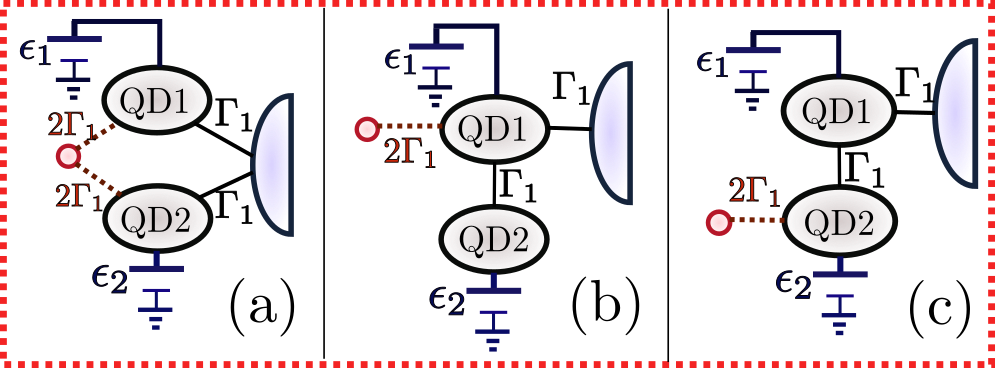
\includegraphics[scale=0.5]{Graficos/MajoranaModels.png}
    \caption{\label{fig:MajoranaModels} (a) Symmetric coupling of the DQD to the lead and the MZM. No inter-dot coupling. (b) T-dot arrangement. (c) Quantum dots coupled in series. 
    }
    %
\end{center}
\end{figure}
%-----------E N D  F I G U R E  2 ------

As mentioned previously, the spin-resolved spectral density (or local density of states LDOS) of each quantum dot provides significant information about the effective tunneling (or not) of a Majorana zero mode into the dot. By comparing the spectral densities for the cases with and without DQD-Majorana couplings, we could identify two generic types of signatures of the Majorana presence in the quantum dots, as follows:

 \begin{itemize}
         \item \textbf{Type I: }  The spin-down LDOS is half of the spin-up LDOS  at the Fermi energy $(\rho_\dw(0)=\rho_\up(0)/2)$. 
         \item \textbf{Type II: } The spin-up spectral density shows a zero mode of height $ \rho_\dw(0) = \frac{0.5}{\pi  \Gamma_1}$ while no such signature appears in the spin-up spectral density. 
     \end{itemize}
     
As we shall see in the following Sections, these two types of signatures appear over a wide range of parameters in our results. Type I often appears when there is a zero-mode in the spin-up L  DOS while Type II typically emerges in when such a spin-up LDOS \change{drops to $0$ at the Fermi energy.} \LUIS{Need to clarify ``destroyed"}\Jesus{I change 'destroyed' by drops to 0}

Hereafter, we shall refer to ``MZM manipulation" the changes in the Majorana signatures in the dot spectral functions induced by the tuning of the dot gate voltages $( \epsilon_1 , \epsilon_2 )$ in the three different setups depicted in Fig.\ref{fig:MajoranaModels}. In each case, we consider definite values of the couplings $\Gamma_2$, $t_{dots}$, $t_1$ and $t_2$, as follows.  In the configuration shown in Fig.\ref{fig:MajoranaModels}(a), we coupled the QD symmetrically to the lead and the MZM by setting $t_1\!=\! t_2$.  Within this setup, we expect the MZM signature to ``split" due to quantum interference and identical signatures should appear in the spectral densities of both dots. We also considered setups in which only one of the dots is coupled directly the MZM or to the metallic lead. Hence, there are only two distinct coupling geometries: either both the MZM and the lead are coupled to the same dot, forming a ``T-junction" or ``side-dot" configuration ($t_{2(1)}\!=\!0$ and $\Gamma_{2(1)}\!=\!0$), as shown in Fig.\ref{fig:MajoranaModels}(b). Alternatively, the MZM can be coupled to one of the dots and the lead to the other, such that the MZM and dots are coupled in series ($t_{1(2)}\!=\!0$ and $\Gamma_{2(1)}\!=\!0$, see Fig.\ref{fig:MajoranaModels}(c)).


%-----------F I G U R E  3 ------
    \begin{figure}[bt]
        \begin{center}
        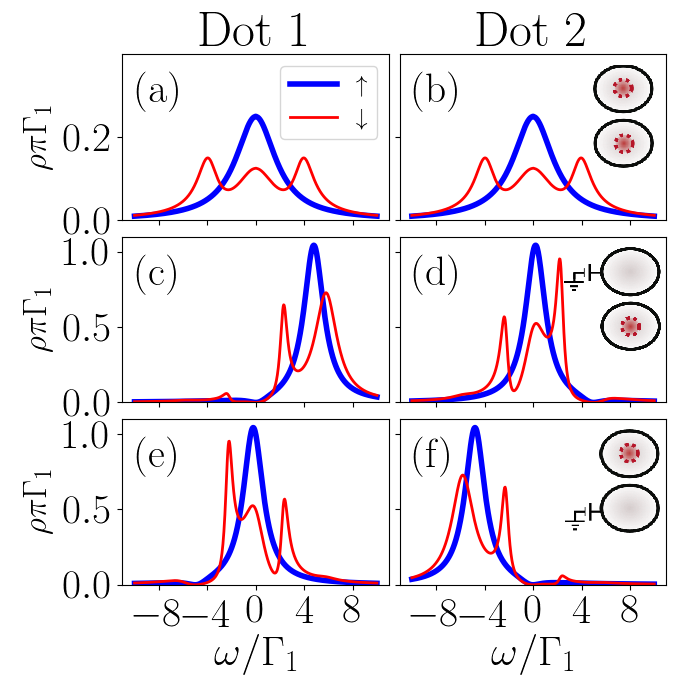
\includegraphics[scale=0.48]{Graficos/t1=t2.png}
       \caption{ \label{fig:t1EQt2}  Spin-resolved spectral densities (LDOS) $\rho_{i \sigma}(\omega)$ for non-interacting  dots $i=1,2$ in the symmetric coupling setup (Fig.\ref{fig:MajoranaModels}(a)). Panels (a), (c) and (e) show $\rho_{1 \sigma}(\omega)$ while panels (b), (d) and  (f) depict $\rho_{2 \sigma}(\omega)$. Each row corresponds to different dot level positions $\ep_1$,$\ep_2$ controlled by gate voltages applied to each dot. (a),(b): $\ep_1=\ep_2=0$. (c),(d): $\ep_1=5\Gamma_1, \ \ep_2 =0$.  (e),(f): $\ep_1=0, \ \ep_2 =-5\Gamma_1$.  Spin-up LDOS $\rho_{i \up}(\omega)$ are marked by bold blue lines while $\rho_{i \dw}(\omega)$ are by thin red lines. Insets show where the MZM signatures, represented by a red dashed circle, are mainly located. 
        }
        %
        \end{center}
    \end{figure}
%-----------E N D  F I G U R E  3 ------



     \subsection{MZM manipulation in non-interacting quantum dots \label{subsect:non-int}}

     % In non-interacting dots $(U=0)$, the density of states at each dot can be obtained from equation \eqref{eq:Density of States} by replacing the green function at \eqref{eq:Green_NonInteracting}. 
     

      %-----------F I G U R E  4 ------
\begin{figure}[bt]
\begin{center}
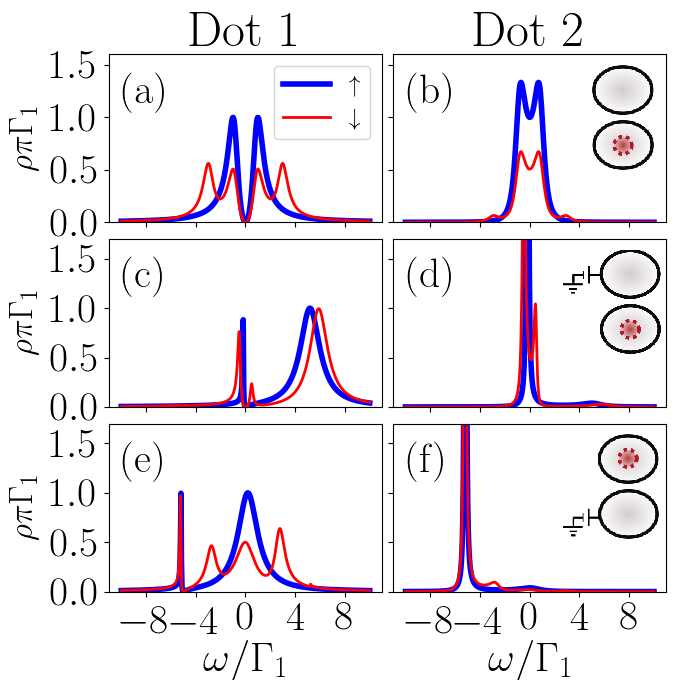
\includegraphics[scale=0.48]{Graficos/t1gt0.png}
\caption{  \label{fig:t1>0}  Spin-resolved spectral densities (LDOS) $\rho_{i \sigma}(\omega)$ for non-interacting  dots $i=1,2$ in the ``T-shaped" configuration (Fig.\ref{fig:MajoranaModels}(b)). Panels (a), (c) and (e): $\rho_{1 \sigma}(\omega)$. Panels (b), (d) and  (f): $\rho_{2 \sigma}(\omega)$. Gate-voltage-controlled energy level  positions are identical as in Fig.\ \ref{fig:t1EQt2}: (a),(b): $\ep_1=\ep_2=0$. (c),(d): $\ep_1=5\Gamma_1, \ \ep_2 =0$.  (e),(f): $\ep_1=0, \ \ep_2 =-5\Gamma_1$.  Spin-up LDOS $\rho_{i \up}(\omega)$ are marked by bold blue lines while $\rho_{i \dw}(\omega)$ are by thin red lines. Insets show where the MZM signatures, represented by a red dashed circle, are mainly located. 
%
}
%
\end{center}
\end{figure}
%-----------E N D  F I G U R E  4 ------


     The non-interacting results for setups (a),(b) and (c) of Fig.\ \ref{fig:MajoranaModels} are shown in Figures \ref{fig:t1EQt2}, \ref{fig:t1>0} and \ref{fig:t2>0} respectively. In all cases, the left (right) panels depict the spectral density  of dot $1$ (dot $2$). Each row represents a different gate voltage configuration in the dots, starting with  $\epsilon_1\!=\!\epsilon_2\!=\!0$ (first row), $\epsilon_1\!=\!5\Gamma_1$, $\epsilon_2\!=\!0$ (second row) and finally $\epsilon_1\!=\!0$, $\epsilon_2\!=\!\!-5\Gamma_1$ (third row). The insets in each row shows where the Majorana signature, represented by a red dashed circle inside the dot, is mainly located. 

%These images will continuously change under the tuning of gate voltages which represents the manipulation of the %Majorana signature.


    
     Figure \ref{fig:t1EQt2} shows results for the symmetric coupling setup (Fig.\ \ref{fig:MajoranaModels}(a)) in the non-interacting regime. For the particle-hole symmetric case (first row), the LDOS for spin-$\dw$ ($\rho_\dw(\omega)$, thin red line) and spin-$\dw$ ($\rho_\up(\omega)$, bold blue line) are identical in both dots, as expected. Notice, however, that the  spin-$\dw$ spectral density (or LDOS) has a 3 peak structure, which is a consequence of the coupling with the Majorana mode. Moreover, the spin-$\dw$ LDOS value at the Fermi energy is \textit{half} of the respective spin-up LDOS value $(\rho_\dw(0) = \frac{1}{2}\rho_\up(0))$, which signals the MZM tunneling into the dots. This Majorana signature is similar to the one observed when a single dot is coupled to a Majorana mode \cite{liu_detecting_2011,vernek_subtle_2014} and falls in our ``type-II" category mentioned above.  We thus may conclude that the MZM is delocalizing into both dots, as if in a ``double slit" configuration. 

More interesting, we find that such delocalization can be reversed (and thus manipulated) by applying gate voltages in the dots. If a positive or negative gate voltage is induced in one of the dots, the spin-$\dw$ LDOS at the Fermi energy can vanish at that dot while the MZM signature $(\rho_\dw(0) = \frac{1}{2}\rho_\up(0)$ remains in the other dot. This is shown in panels (c)-(f) of Fig.\ \ref{fig:t1EQt2} for the case of positive (Fig.\ \ref{fig:t1EQt2}(c-d) and negative (Fig.\ \ref{fig:t1EQt2}(e-f) gate voltages. 
%
%This means that the MZM is actually being induced to "leave" this dots and leak into the other dot by the gate %voltage activation. This first example of MZM manipulation. 


    The location of the MZM signature can also be controlled by quantum interference, as illustrated in panels (a) and (b) of Fig.\ \ref{fig:t1>0}. Here, the MZM is coupled directly only to dot 1, which is then coupled to the lead, while dot 2 is coupled only to dot 1 via the inter-dot tunneling term (``side-dot'' configuration, see Fig.\ \ref{fig:MajoranaModels}(b). Interestingly, if the energy level of dot 2 is fixed to be in resonance with the Fermi energy of the lead, quantum interference causes the spectral function in dot 1 to \textit{vanish} at the Fermi level (Fig.\ \ref{fig:t1>0}(a), while a type-I MZM signature $(\rho_\dw(0) = \frac{1}{2}\rho_\up(0))$ appears in dot 2 only (Fig.\ \ref{fig:t1>0}(b). This interference-induced MZM signature in dot 2 is robust against shifts in dot 1's gate voltage, as depicted in Figs.\ \ref{fig:t1>0}-c \& d.  While dot 1's LDOS is pinned at zero at the Fermi energy, dot 2's spin-$\dw$ LDOS exhibits a robust zero-mode of height $\frac{0.5}{\pi \Gamma}$, which is a type-II MZM signature. 

This qualitative picture is radically altered when dot 2's gate voltage is shifted away from zero (Figs.\ \ref{fig:t1>0}(e)\&(f)). In this case, dot 2 is no longer in resonance with the leads, which changes the interference conditions such that dot 1 spectral function is no longer pinned at zero. The plots clearly show that the MZM signature, previously located in dot 2, now appears in dot 1. Moreover, the spin-up and spin-$\dw$ LDOS in dot 1 become very similar to the spectral densities observed in the case of a single dot \cite{liu_detecting_2011,vernek_subtle_2014}, which indicates that dot 2 is essentially decoupled from the MZM. 




 %-----------F I G U R E  5 ------
\begin{figure}[t]
\begin{center}
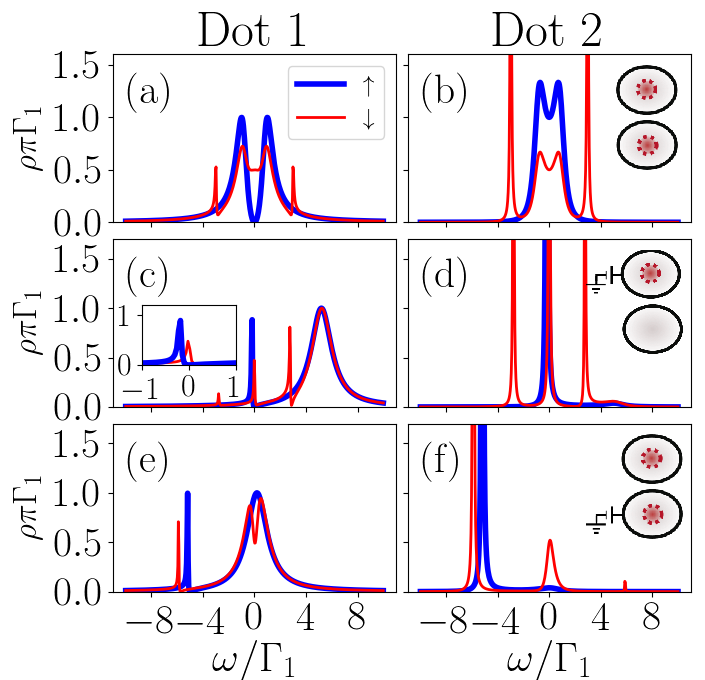
\includegraphics[scale=0.48]{Graficos/t2gt0.png}
\caption{  \label{fig:t2>0} Spin-resolved spectral densities (LDOS) $\rho_{i \sigma}(\omega)$ for non-interacting  dots $i=1,2$ in the ``in-series'' configuration (Fig.\ref{fig:MajoranaModels}(c)). 
Panels (a), (c) and (e): $\rho_{1 \sigma}(\omega)$. Panels (b), (d) and  (f): $\rho_{2 \sigma}(\omega)$. Gate-voltage-controlled energy level  positions are identical as in Fig.\ \ref{fig:t1EQt2}: (a),(b): $\ep_1=\ep_2=0$. (c),(d): $\ep_1=5\Gamma_1, \ \ep_2 =0$.  (e),(f): $\ep_1=0, \ \ep_2 =-5\Gamma_1$.  
Spin-up LDOS $\rho_{i \up}(\omega)$ are marked by bold blue lines while $\rho_{i \dw}(\omega)$ are by thin red lines. Insets show where the MZM signatures, represented by a red dashed circle, are mainly located. \change{Inset in (c): Detailed low-energy features.}
%
}
%
\end{center}
\end{figure}
%-----------E N D  F I G U R E  5 ------
     



    Finally, we consider the ``in-series'' configuration of  Fig.\ \ref{fig:MajoranaModels}(c), in which is similar to the ``side-dot''  configuration (Fig.\ \ref{fig:MajoranaModels}(b)) except for the fact that the (spin-$\dw$) MZM is coupled only to dot 2. Thus, results for the spin-up LDOS are identical to those shown in Fig.\ \ref{fig:t1>0}. However, the MZM signatures in the spin-$\dw$ LDOS are quite distinct. As an example, when both dots are in resonance with the lead (Fig.\ \ref{fig:t2>0}(a) and (b)), the spin-$\dw$ LDOS does not vanish at $\omega\!=\!0$ as in the previous case. Instead, both dots show $(\rho_\dw(0)=\frac{0.5}{\pi \Gamma})$, which leads to MZM signatures of type-I in dot 2 and type-II in dot 1.
    
% A shift in dot 1's gate voltage erases \change{the MZM signature in dot 2, but not in dot $1$,} as shown in Figs.\ \ref{fig:t2>0}(c) and (d). Interestingly, the MZM signatures are robust against changes in the dot 2's gate voltage (Figs.\ \ref{fig:t2>0}(e) and (f) , but now the MZM signature types are switched: QD1 shows a type-I signature, while QD2 shows a type-II one.  \change{In addition, note the Majorana signature remains stable inside the dot that is directly attached to the lead at all gate voltage configurations.}

\change{Moreover, the MZM signature inside dot one is present at all configurations, despite the fact that it is not directly attached to the MZM. A shift in dot 1's gate voltage erases \change{the MZM signature in dot $2$, but not in dot $1$,} as shown in Figs.\ \ref{fig:t2>0}(c) and (d). On the other hand, the MZM signatures are robust against changes in the dot 2's gate voltage (Figs.\ \ref{fig:t2>0}(e) and (f) , but now the MZM signature types are switched: QD1 shows a type-I signature, while QD2 shows a type-II one.}  


\LUIS{I think there is a MZM signature in the dot 1 in Fig.\ \ref{fig:t2>0}(c). Please add this to the inset.}  

    % With the MZM coupled only to the second dot, it is impressive that a Majorana signature of height $\frac{0.5}{\pi \Gamma}$ appears it the first dot despite there is no direct connection  between them. 
    % On the other hand, if the Majorana mode is attached to the second dot in the previous arrangement, then both dots will exhibit a majorana signature. However, the signature in dot 1 is different from the others. The spin-$\dw$ LDOS reveals the emergence of a zero mode with height close to $5.2$ (such that $\pi  \Gamma_1 \rho_\dw(0) = 0.5$). However the spin-up LDOS remains equal to $0$. This new type of majorana signature is the result of an indirect connection between QD1 and the majorana mode attached t the second dot. As in the previous case, turning on the gate voltage in dot $1$ destroys the majorana signature in both dots. Instead, if the gate voltage in dot $2$ is turned on, both dots will preserve the Majorana signature. 

    %  \noindent The state of these signatures for each of these stated is depicted in Fig.\ \ref{fig:MajoranaModels}. A solid filled red circle inside the dot represents the appearance of a Type I Majorana signature, on the othere hand a dashed filled red circle represents the presence a  Type II Majorana signature. The obscure dashed circle represents a vanishing majorana signature due to an applied gate voltage or by quantum interference.

\subsection{Interacting dots: MZM-mediated indirect exchange \label{subsec:IndirectExchange}}


We now turn to the more realistic case of quantum dots in the Coulomb blockade regime where local electron-electron interaction terms dominate the spectral function. We consider the dots to be in an odd-$N$ Coulomb blockade valley where Kondo correlations are dominant at low-temperatures. The local Coulomb energy in the dots is accounted for by the terms $\frac{U_i}{2}(\sum_{\sigma} \hat{n}_{i\sigma}-1)^{2}$ in Eq.\ \eqref{eq:H_DQD}. For simplicity, we consider equal Coulomb repulsion energies $(U_1 \!=\! U_2 \equiv U)$ for both dots. For concreteness, the NRG calculations were performed with $U \!=\! 17.3\Gamma_1$ in both dots and a half-bandwidth of the lead electrons set at $D=2U=34.6\Gamma_1$. 


Let us review some of the main features of the spectral densities of the dots in the absence of the MZM coupling. For a single dot coupled to a metallic lead, the Kondo effect is characterized by the appearance of a sharp resonance in the spectral function near the Fermi energy with a width of order $k_B T_K \!\sim\! \sqrt{U \Gamma_1} \exp \left[- \pi\frac{|\epsilon_1| |\epsilon_1 + U|}{U \Gamma_1}  \right]$. Here, $T_K \ll U$ is the Kondo temperature  of the system \cite{hewson_kondo_1997}, which will be largest at the particle-hole symmetric point (phs)  $\epsilon_1 \!=\!-\frac{U}{2}$. In the case of two dots at phs ($\left(\epsilon_{di}\!=\! -\frac{U_i}{2}\right)$), both symmetrically coupled to a single lead ($\Gamma_1\!=\!\Gamma_2$), there will be an additional effective exchange interaction between the dots mediated by the lead \cite{Liao:JournalofMagnetismandMagneticMaterials:377:354-361:2015}. Such exchange will compete with the antiferromagnetic Kondo coupling, producing a three-peak structure in the spectral density of both dots. 

Figure \ref{fig:NRG_Majorana}(a) show the spectral functions for both dots in this case. At large energies, the spectral density displays Hubbard peaks at $\omega \sim \epsilon_{di} \pm 8.6\Gamma_1 = \pm \frac{U}{2}$, representing the single-particle hole- and electron-excitations and whose width is of order $\sim 4\Gamma_1$. At low energies, the spin-independent spectral densities show a central Kondo peak accompanied by indirect-exchange-induced satellite peaks at \change{ $\omega \sim \pm 3.46 \Gamma^2_1/U$, giving an energy separation that scales as $\sim \Gamma^2_1/U$ (see also insets in Fig.\ \ref{fig:NRG_Majorana}(a)) \cite{Liao:JournalofMagnetismandMagneticMaterials:377:354-361:2015}}. 



%In the absence of the  sufficiently low temperature the system will exhibit the characteristic Kondo peaks at the Fermi energy \citet{wilson_renormalization_1975}. The coexistence of Kondo and Majorana zero modes is still a point of contention in the area and one of the objectives of this part of the project


     %-----------E N D  F I G U R E  6 ------    
        \begin{figure}[bt]
        \begin{center}
        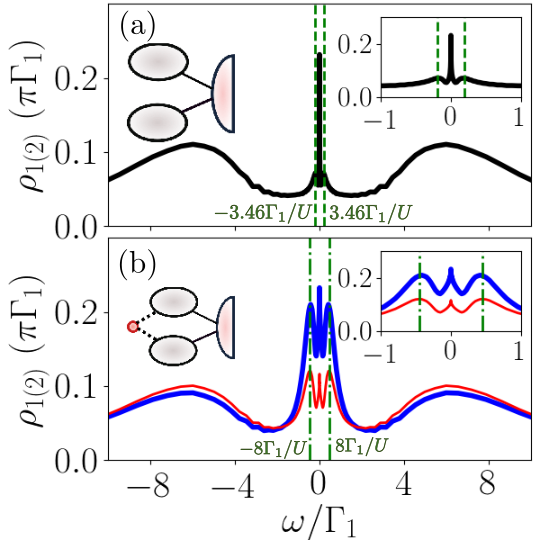
\includegraphics[width=1.0\columnwidth]{Graficos/NRG_t1zero_t1eqt2.png}
        \caption{  \label{fig:NRG_Majorana} Spectral density (LDOS) for interacting dots ($U_1\!=\!U_2\!=\!17.3 \Gamma_1$) in the symmetric coupling configuration ($\Gamma_1\!=\!\Gamma_2$ and $t_1\!=\!t_2)$.  (a) Uncoupled MZM ($t_1\!=\!t_2\!=\!0$). Spin up and down spectral densities are identical and given by the black line. (b) Coupled MZM ($t_1\!=\!t_2\!=\!\Gamma_1$):S spin-up (bold blue lines) and  spin-down (thin red lines) spectral densities are shown. Insets: Magnification of the low-energy region. 
        }
        \end{center}
        \end{figure}
    %-----------E N D  F I G U R E  6 ------

Such exchange-driven three-peak structure remains when the MZM is coupled to the system in the symmetric coupling configuration, as shown in Figure\ \ref{fig:NRG_Majorana}(b). More striking is that the indirect-exchange splitting between the dots increases considerably with the MZM coupling \change{up to $\sim \pm 8\Gamma_1^2/U$ : our calculations show that the peak separation of the Majorana satellites increases quadratically with the MZM coupling $t_1\!=\!t_2$as $4t_1^2/U$  and this effect enters in superposition with the indirect-exchange-induced satellites in Fig.\ \ref{fig:NRG_Majorana}(a)  \LUIS{Jesus: please check if it goes as $\sim t \Gamma_1/U$ or something else}}. This indicates a MZM-mediated spin-spin correlation between the quantum dots. Thus, the coupling to a spin-down-polarized MZM (which is the case) affects the spin-up component of the spectral densities through this indirect spin-spin interaction. Additional details of these interesting features will be discussed elsewhere \LUIS{Add a citation to a paper in preparation...}\Jesus{I don't know how to do this...}.

 %\cite{ruderman_indirect_1954,kasuya_theory_1956,yosida_magnetic_1957} 
%\LUIS{Ok, we need to add that discussion on the atomic limit. I would not call this RKKY. It is a hybridization %between the dots!} 



    \subsection{MZM manipulation in interacting dots \label{subsec:Interacting}}



 %-----------F I G U R E  7 ------
\begin{figure}[bt]
\begin{center}
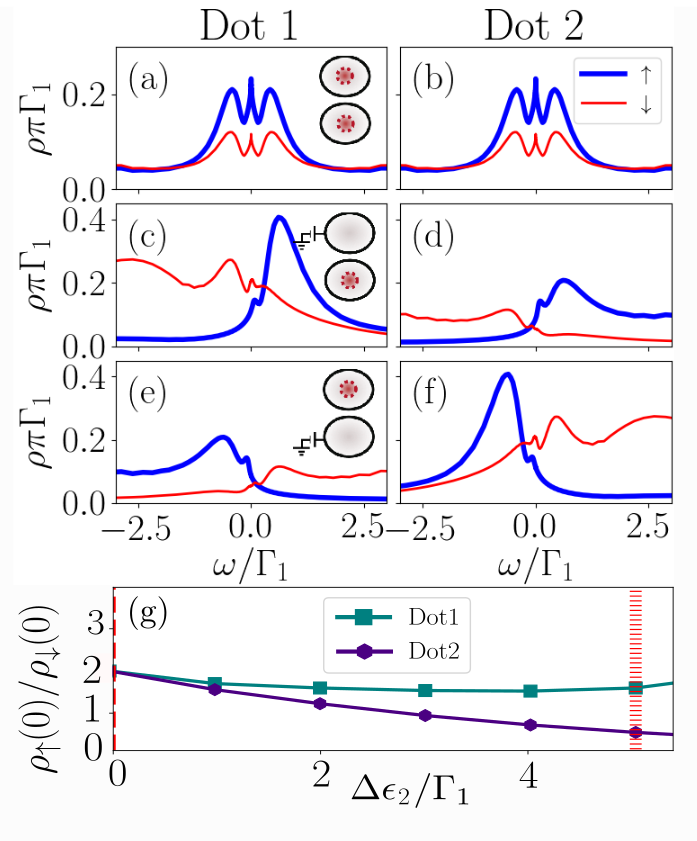
\includegraphics[scale=0.45]{Graficos/N2t1=t2.png}
\caption{ \label{fig:Nt1=t2} Spin-resolved spectral densities  $\rho_{i \sigma}(\omega)$ for \textit{interacting}  dots $i=1,2$ with $U_1\!=\!U_2\!=\!17.3 \Gamma_1$. Here we consider the symmetric coupling configuration shown in Fig.\ref{fig:MajoranaModels}(a). Panels (a) and (b) show $\rho_{1 \sigma}(\omega)$ and $\rho_{2 \sigma}(\omega)$ respectively for the particle-hole symmetric case $\ep_1\!=\!\ep_2\!=\!-U/2$. Panels (c) and (d) show $\rho_{1 \sigma}(\omega)$ and $\rho_{2 \sigma}(\omega)$ for $\ep_1\!=\!-U/2+\Delta \ep_1$ and $\ep_2\!=\!-U/2$ with $\Delta \ep_1=5\Gamma_1$.  Symmetrically, in panels (e) and (f), $\ep_2\!=\!-U/2+\Delta \ep_2$ and $\ep_1\!=\!-U/2$ with $\Delta \ep_2=-5\Gamma_1$ .Insets show where the MZM signatures, represented by a red dashed circle, are mainly located.  (g): Evolution of $\rho_{i \dw(0)}/\rho_{i \up(0)}$ vs $\Delta \ep_2$, for $\ep_1\!=\!-U/2$. Dashed line: $\Delta \ep_2 =0$ as in (a),(b). Barred  line: $\Delta \ep_2 =5\Gamma_1$ as in (c),(d). 
 \LUIS{Jesus, please check these parameters. Here, panel (e) shows a  plot $\Delta \ep_1$ but I think is versus $\Delta \ep_2$ as in Fig. 5.8 of the dissertation.} \Jesus{SOLVED}
}
%
\end{center}
\end{figure}
%-----------E N D  F I G U R E  7 ------




Moreover, the system presents a Majorana signature characterized by a type-I MZM signature $\rho_\dw(0) = \frac{1}{2}\rho_\up(0)$. Note, that in this case the MZM signature coexists with the Kondo peak in the DQD as already predicted in Refs. \cite{lee_kondo_2013,ruiz-tijerina_interaction_2015} for a MZM coupled to a single quantum dot. As in that case, here both Kondo and MZM signatures occur in low-energy part of the spectral function $\omega \lesssim \Gamma_1$, as illustrated in the inset of Fig.\ \ref{fig:NRG_Majorana}(b). Within this scale, we can trace some interesting parallels with the non-interacting regime. 

As an example, Fig.\ \ref{fig:Nt1=t2} shows the NRG results for the symmetric setup in Fig.\ \ref{fig:MajoranaModels}(a). As in the non-interacting case (Fig.\ \ref{fig:t1EQt2}), type-I MZM  signatures appear in both dots.  These signatures can be manipulated by tuning one of the dot's gate voltage to induce the MZM signature to appear only in the other dot. The LDOS at figures Fig.\ \ref{fig:Nt1=t2}(d) shows a type-I MZM  signature with $\rho_\dw(0) \approx \frac{1}{2}\rho_\up(0)$. This MZM signature is stable against gate-voltage-induced energy shifts in dot 2 away from particle-hole symmetry ($\Delta \ep_2 \equiv \ep_2+U/2$) in the range $\Delta \ep_2 \lesssim 6\Gamma_1$ (see Fig.\ \ref{fig:Nt1=t2}(e)). For larger values of $\Delta \ep_2$, dot 2 enters the mixed-valence regime and the Coulomb peak originally located at $\omega \sim \pm 8.7 \Gamma_1$ for $\Delta \ep_2\!=\!0$ now overlaps with the Fermi energy and both Majorana and Kondo signals are lost.

  



 %-----------F I G U R E  4 ------
\begin{figure}[bt]
\begin{center}
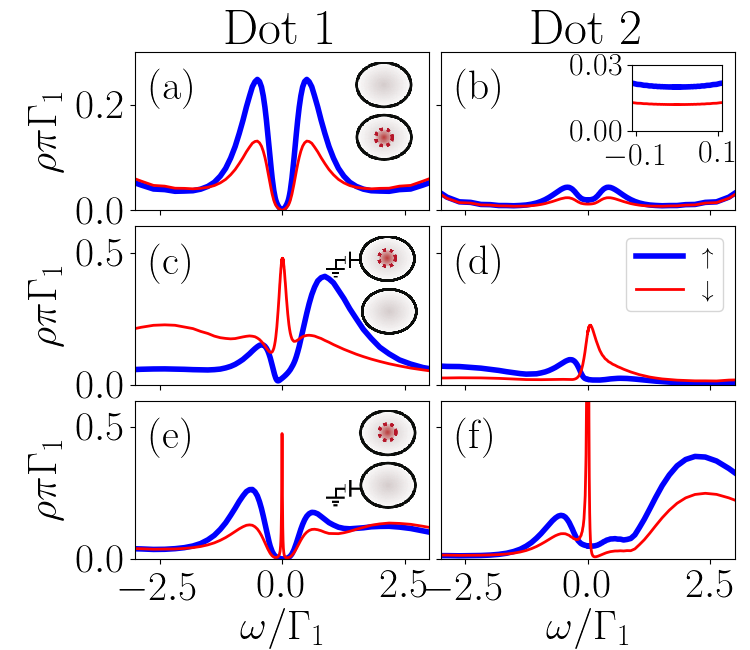
\includegraphics[scale=0.45]{Graficos/b_Nt1gt0.png}
\caption{  \label{fig:Nt1>0} Spin-resolved spectral densities $\rho_{i \sigma}(\omega)$ for interacting  dots $i=1,2$ in the ``T-shaped" configuration (Fig.\ref{fig:MajoranaModels}(b)). Panels (a), (c) and (e): $\rho_{1 \sigma}(\omega)$. Panels (b), (d) and  (f): $\rho_{2 \sigma}(\omega)$. Energy level  positions are identical as in Fig.\ \ref{fig:Nt1=t2}: (a),(b): $\ep_1\!=\!\ep_2\!=\!-U/2$. (c),(d): $\ep_1=-U/2+5\Gamma_1, \ \ep_2 =-U/2$.  (e),(f): $\ep_1=-U/2, \ \ep_2 =-U/2-5\Gamma_1$.  Spin-up LDOS $\rho_{i \up}(\omega)$ are marked by bold blue lines while $\rho_{i \dw}(\omega)$ are by thin red lines. Insets show where the MZM signatures, represented by a red dashed circle, are mainly located. Inset in (b): Detail of the low-energy features.
%
}
%
\end{center}
\end{figure}
%-----------E N D  F I G U R E  4 ------



    %Poisoning.

 Results for the interacting ``side-dot'' set-up (Fig.\ \ref{fig:MajoranaModels}(b)) are shown in Fig.\ \ref{fig:Nt1>0}. As in the non-interacting case, the spin-up spectral density of dot 1  vanishes at the Fermi level due to single-particle quantum interference, as shown in Fig.\ \ref{fig:Nt1>0}(a). In dot 2, the spectral density is drastically reduced at the Fermi level, but it remains non-zero (Fig.\ \ref{fig:Nt1>0}(b) and inset), while still showing a type-I MZM signature, namely, \change{$\rho_\dw(0)=\frac{\rho_\up(0)}{2}$}. This picture is qualitative similar to the non-interacting case discussed previously, but it begs the question of what is the fate of the Kondo resonance in the dots in this configuration.
%L Here



    
  %-----------F I G U R E  5 ------
\begin{figure}[bt]
\begin{center}
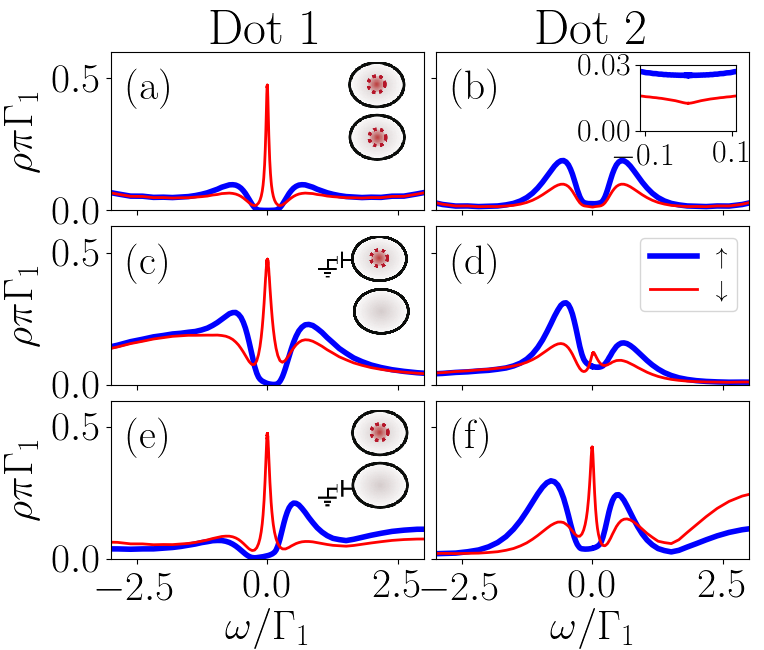
\includegraphics[scale=0.45]{Graficos/b_Nt2gt0.png}
\caption{  \label{fig:Nt2>0} Spin-resolved spectral densities $\rho_{i \sigma}(\omega)$ for interacting  dots $i=1,2$ in the ``in-series" configuration (Fig.\ref{fig:MajoranaModels}(c)). Panels (a), (c) and (e): $\rho_{1 \sigma}(\omega)$. Panels (b), (d) and  (f): $\rho_{2 \sigma}(\omega)$. Energy level  positions are identical as in Fig.\ \ref{fig:Nt1=t2}: (a),(b): $\ep_1\!=\!\ep_2\!=\!-U/2$. (c),(d): $\ep_1=-U/2+5\Gamma_1, \ \ep_2 =-U/2$.  (e),(f): $\ep_1=-U/2, \ \ep_2 =-U/2-5\Gamma_1$.  Spin-up LDOS $\rho_{i \up}(\omega)$ are marked by bold blue lines while $\rho_{i \dw}(\omega)$ are by thin red lines. Insets show where the MZM signatures, represented by a red dashed circle, are mainly located. Inset in (b): Detail of the low-energy features.
%
}
%

\end{center}
\end{figure}
%-----------E N D  F I G U R E  5 ------


To try and answer this question, we note that a similar interplay between Kondo physics and single-particle interference on a T-shaped double dot geometry has been studied in earlier works by one of us \cite{Silva:096603:2006,dias_da_silva_transmission_2008,DiasdaSilva:Phys.Rev.Lett.:116801:2017}. It has been established that, for the case of the dot coupled to the lead (dot 1, in the present case) being non-interacting, its spectral density vanishes at the Fermi energy, whilst the spectral density in the second dot (dot 2) shows a ``splitted" Kondo resonance for strong enough inter-dot coupling. The Kondo screening in this second dot, however, is still present. In fact, the Kondo temperature \textit{increases} with the interdot coupling \cite{Silva:096603:2006,DiasdaSilva:Phys.Rev.Lett.:116801:2017}. Here the situation is slightly different as dot 1 is also interacting but we believe the analogy still holds. This picture would explain why the up and down components of the spectral density in dot 2 do not vanish at the Fermi energy (although they are quite suppressed) while still showing the MZM type-I signature ($\rho_\dw(0)=\frac{1}{2}\rho_\up(0)$).




When gate voltages are applied in either dot 1 or dot 2, a MZM signature appears in dot 1. This is shown in Figs.\ \ref{fig:Nt1>0}(c)-(f): a type-II MZM signature ($\rho_\dw(0)=\frac{0.5}{\pi \Gamma_1}$, $\rho_\up(0) \approx 0$) appears in dot 1 while neither type-I or type-II signatures are evident in dot 2. This is clearly distinct from the non-interacting case , in which a shift in the gate voltage of dot 1  (Figs.\ \ref{fig:t1>0}(c)-(d)) leads to a type-\change{II} \LUIS{or is it type-II?}\Jesus{It is type II} MZM signature in dot 2 and vice-versa \Jesus{vice-versa?. Not sure what it means} . When interactions are present and the system is tuned out of the particle-hole symmetric point, no clear type-I or type-II MZM signatures appear in dot 2's spectral density (see  Figs.\ \ref{fig:Nt1>0}(d) and (e)). Instead, Fano-like resonances near the Fermi energy with comparable widths are present in the spin down spectral densities. We attribute those to single-particle interference with dot 1 since the heights are not set at  $\rho_\dw(0)=\frac{0.5}{\pi \Gamma_1}$.







   Finally, Fig.\ \ref{fig:Nt2>0} depicts the NRG results for the ``series'' configuration shown in Fig.\ \ref{fig:MajoranaModels}(c). In this configuration, the MZM is coupled directly to dot 2 only. \change{Like in the \textit{non-interacting} case}, the strongest MZM signatures (type-II, in this case) occur in the spectral properties \textit{of dot 1 and not in those of dot 2}.  As an illustration, Figs.\ \ref{fig:Nt2>0}(a),(c) and (e) show robust zero-energy peaks in the spin down spectral densities of dot 1 obeying $\rho_\dw(0)=\frac{0.5}{\pi \Gamma_1}$ while $\rho_\up(0) \approx 0$. The strong difference between spin up and down spectral densities clearly identifies this as a MZM signature rather than a Kondo peak. 
   
The type-II MZM signature remains in dot 2 despite changes in gate voltages in either dot 1  (Fig.\ \ref{fig:Nt2>0}(c)) or dot 2 (Fig.\ \ref{fig:Nt2>0}(e)). Moreover,  a type-\change{I} \Jesus{This one is type one} MZM signature also appears in dot 2  in the particle-hole symmetric case, as depicted in Fig.\ \ref{fig:Nt2>0}(b). Away from particle-hole symmetry, the MZM traces in the spectral properties of dot 2 are less clear. While a shift in the dot 1 energy $\Delta \ep_1=+5 \Gamma_1$ has little effect in the dot 2 spectral density (Fig.\ \ref{fig:Nt2>0}(b)), changing the energy of dot 2 by an amount  $\Delta \ep_2=-5 \Gamma_1$ gives a zero-energy peak in the dot 2 spin down spectral density (Fig.\ \ref{fig:Nt2>0}(d)). \change{Although these dot 2 spectral properties near zero energy are close in meeting the type-II MZM signature condition for this case ($\rho_\dw(0)=\frac{0.5}{\pi \Gamma_1}$ and $\rho_\up(0) \approx 0$), we observed that this signature is not universal. Indeed, $\rho_\dw(0)$ varies considerably with  $\epsilon_2$. Therefore we cannot categorize it as Majorana signature.} 
\LUIS{I think this can be understood as a zero mode in dot 2 as well}    
  \LUIS{I think there is a MZM signature in the dot 2 in Fig.\ \ref{fig:Nt2>0}(f). Please add this to the inset. Then Figs. \ref{fig:t2>0} and \ref{fig:Nt2>0} show the same pattern. } \Jesus{This is not the case, I added the answer}

One way to understand these results is to use the ``Majorana leaking" analogy of Ref. \cite{vernek_subtle_2014}. In the series configuration of Fig.\ \ref{fig:MajoranaModels}(c), both dots can be though as non-topological ``extensions" of the Kitaev chain, with dot 1 being the ``last site" or the ``edge". Thus, due to the leaking of the MZM to the neighboring sites (as it is the case of a MZM attached to a single quantum dot \cite{vernek_subtle_2014,ruiz-tijerina_interaction_2015}), it would be expected that  edge-mode signatures in dot 1 would be quite robust against changes in gate voltages. 



%On the other hand, this interpretation fails in the non-interacting case. On the other hand, there is a significant zero-mode in the spin-$\dw$ LDOS. This mode was not identified as a potential Majorana signature since it increases when $\Delta \ep_2$. 


%---------------------------------------------------------------------------  
\section{Concluding remarks}
\label{sec:Conclusions}


In this paper, we have addressed the following question: can one manipulate and detect Majorana zero-modes (MZMs) in an all-electric set-up using semiconductor double quantum dots? To this end, we considered a minimal model of a MZM coupled to a double quantum dot (DQD) and metallic leads and calculated the spectral signatures in both strongly- and weakly-interacting regimes. By comparing exact analytical solutions in the non-interacting system and numerical renormalization-group results for interacting quantum dots, we were able to characterized the displacements of the MZM inside the double quantum dot for the three setups in Fig.\ \ref{fig:MajoranaModels}. 

Our results for both weakly- and strongly-interacting regime show that gate-voltage tuning in the dots allows for an effective manipulation of the tunneling of the MZM into the DQD system. By considering different MZM-DQD coupling geometries (``symmetric'', ``T-shaped'' and ``in-series'') we found that the presence or not of the MZM in each dot can be monitored by two types of signatures in the spectral density (or local density of states) of the dots.

In the symmetric configuration, the MZM is equally coupled to both dots. As in a ``double slit'' set up, the MZM signature will appear in \textit{both} dots if the gate voltages are tuned to the particle-hole symmetric (phs) point. By changing the gate voltage in one of the dots (the equivalent of ``closing one of the slits''), the MZM signature will move to the other dot. In the ``T-shaped'' configuration, when the MZM is directly coupled only to dot 1, the MZM signature will appear only in one of the dots: either dot 2 (at phs or if a gate voltage is applied to dot 1) or in dot 1, when a gate voltage is applied to dot 2. 

Finally, we considered a configuration with the MZM coupled ``in-series'' with both dots, which is closely connected with recent design proposals for  topological quantum computational circuits involving MZMs \cite{karzig_scalable_2017}. In this case, there is a robust MZM signature in the ``far dot'', (the one not directly coupled to the MZM) for all gate voltage configurations, while the MZM signature in the dot directly coupled to the MZM can be manipulated via gate-voltage tuning.


Electron-electron interactions will add some interesting effects to this picture. First, there will be the appearance of a Kondo resonance in the dots, which will split due to the indirect exchange between the dots mediated by the leads.  More interestingly, we find that the coupling of the dots to the (spin-polarized) MZM will also contribute to the indirect exchange, thus creating a MZM-mediated spin exchange between the dots.  These indirect exchange effects are more prominent in the symmetric configuration, where satellite peaks in the spectral density reflect the combined Kondo-Majorana physics at low energies. 



%
%
%In this system, the spin-up zero mode at QD1 (The Kondo peak if the system is interacting) is destroyed by quantum interference with the second dot, as shown in Fig.\ .\ref{fig:MajoranaModels}(b). This interference will also destroy the MZM in the first dot but a type I Majorana signature will still appear in the second dot. The Majorana mode can be induced to tunnel back into the first dot if a gate voltage is applied on the second dot. This signature is visible at very low energies (bellow $0.1\Gamma_1$) in interacting case. 




\begin{acknowledgments}
The authors thank Edson Vernek for enlightening discussions.  L.G.G.V.D.S. acknowledges financial support by CNPq (grants No. 307107/2013-2 and 449148/2014-9), and FAPESP (grant No. 2016/18495-4).
\end{acknowledgments}

% \LUIS{Only ONE bib file}

%---------------------- Apendix A------------------------


%-----------------------------------------------------------



 \appendix

 
 \section{Computation of the Green Function  \label{sec:Appendix_alg}}


 The spectral representation of the retarded Green function  \cite{zubarev_double-time_1960} associated to two fermion operators $A(t)$ , $B(t')$ is 
 \begin{equation}
 \Green{A,B} \equiv-i \int e^{i \omega t} \Theta(t)\left\langle\{A(t), B(0)\}\right\rangle d t. 
\end{equation}
Using the equations of motion technique we obtain the following relation \cite{zubarev_double-time_1960}
\begin{equation}
    \omega\Green{A,B}=\delta_{A^{\dagger},B}+\Green{\left[A,H\right],B}.
    \label{eq:Transport}
\end{equation}
\noindent We apply this expression to Hamiltonian $H$ \eqref{eq:Model}, with $B \equiv d^\dagger_{1\dw}$ and $A$ varying between the fermion operators $d^\dagger_{i\dw}, f^\dagger_\dw,c^\dagger_{k\dw}, d_{i\dw},f_\dw ,c_{k\dw}$. Taking $(\omega,t_1,t_2,\epsilon_1 \ldots)$ as fixed parameters, we obtain a closed linear system of $8$  equations with $8$ variables of the form $\Green{A,d^\dagger_{1\dw}}$. Hence this system has a unique solution. 

We are interested in computing an analytic expression for $\Green{d_{1\dw},d^\dagger_{1\dw}}$. The expected solution is a polynomial fraction of degree $8$, whose complexity depends on the number of couplings between the fermion operators. The method described in this paper borrows ideas from graph theory to simplify the Gauss-Jordan elimination process \citet{spielman_algorithms_2010}. We use this method to deduce a simple algorithm to solve the equations of motion of Hamiltonian $H$ \eqref{eq:Model}.  


% we obtain a system of $64$ equations.  Nonetheless, it is possible to simplify its the complexity by fixing $B = d^\dagger_{1\dw}$ and allowing the operator $A$ to vary among all the other fermion operators. The remaining system of $8$ equations is closed since the $B$ component does not vary among the EOM \eqref{eq:Transport}

Before describing the general procedure, note that  the equations of motion \eqref{eq:Transport} for $A$ equal to $f_\dw$ and $f^\dagger_\dw$ are  
\begin{align}
        \omega\Green{f_{\downarrow},d_{1\downarrow}^{\dagger}}&= \omega\Green{f^\dagger_{\downarrow},d_{1\downarrow}^{\dagger}} \\
        &= \sum_{i=1}^2 \frac{t_i}{\sqrt{2}}\left(\Green{d_{i\downarrow},d_{1\downarrow}^{\dagger}}-\Green{d_{i\downarrow}^{\dagger},d_{1\downarrow}^{\dagger}}\right). 
\end{align}

% \begin{align}
%         \left(\omega-\epsilon_{M}\right)\Green{f_{\downarrow},d_{1\downarrow}^{\dagger}}&= \sum_{i=1}^2 \frac{t_i}{\sqrt{2}}\left(\Green{d_{i\downarrow},d_{1\downarrow}^{\dagger}}-\Green{d_{i\downarrow}^{\dagger},d_{1\downarrow}^{\dagger}}\right), \\
%     \left(\omega+\epsilon_{M}\right)\Green{f_{\downarrow}^{\dagger},d_{1\downarrow}^{\dagger}}&=\sum_{i=1}^2\frac{t_i}{\sqrt{2}}\left(\Green{d_{i\downarrow},d_{1\downarrow}^{\dagger}}-\Green{d_{i\downarrow}^{\dagger},d_{1\downarrow}^{\dagger}}\right).
% \end{align}
\noindent Since $\Green{f_{\downarrow}^{\dagger},d_{1\downarrow}^{\dagger}} = \Green{f_{\downarrow},d_{1\downarrow}^{\dagger}} $ it is possible to eliminate the variable $\Green{f_{\downarrow}^{\dagger},d_{1\downarrow}^{\dagger}} $ from the system even before starting the Gauss-Jordan elimination. 

Writing the remaining EOMs \eqref{eq:Transport} for $A$ varying between  $d^\dagger_{i\dw},c^\dagger_{k\dw}, d_{i\dw},f_\dw ,c_{k\dw}$,   we obtain the following linear system
\begin{equation}
    \mathcal{T} \vec{G}_{d^\dagger_1} = \hat{e}_1,
\end{equation}

\noindent where $\hat{e_1}$ is the vector with entries  $\hat{e}_{1_n} =\delta_{1n}$, $\mathcal{T}$ is the  matrix 
\begin{equation}
\left[\begin{array}{ccccccc}
\omega-\epsilon_{1} & -V_{1}^{*} & -t_{dots} & -t_{1} & 0 & 0 & 0\\
-V_{1} & \omega-\epsilon_{k} & -V_{2} & 0 & 0 & 0 & 0\\
-t_{dots}^{*} & -V_{2}^{*} & \omega-\epsilon_{2} & -t_{2} & 0 & 0 & 0\\
-t_{1}^{*} & 0 & -t_{2}^{*} & \omega-\epsilon_{M} & -t_{2}^{*} & 0 & -t_{1}\\
0 & 0 & 0 & -t_{2} & \omega+\epsilon_{2} & V_{2}^{*} & t_{dots}^{*}\\
0 & 0 & 0 & 0 & V_{2} & \omega+\epsilon_{k} & V_{1}\\
0 & 0 & 0 & -t_{1} & t_{dots} & V_{1}^{*} & \omega+\epsilon_{1}
\end{array}\right],
\label{eq:TransportMatrix}
\end{equation}
 \noindent  and $\vec{G}_{d^\dagger_1}$  is the column vector
%  wit indices
%  $\Green{d_{\mathbf{1\downarrow}},d_{1\downarrow}^{\dagger}},\Green{c_{k\downarrow},d_{1\downarrow}^{\dagger}},\Green{d_{2\downarrow},d_{1\downarrow}^{\dagger}}$
% %  $ \Green{d_{\mathbf{1\downarrow}},d_{1\downarrow}^{\dagger}},\Green{c_{k\downarrow},d_{1\downarrow}^{\dagger}},\Green{d_{2\downarrow},d_{1\downarrow}^{\dagger}},\Green{f_{\downarrow}$
 
 \begin{align*}
    \Big[ &  \Green{d_{\mathbf{1\downarrow}},d_{1\downarrow}^{\dagger}},\Green{c_{k\downarrow},d_{1\downarrow}^{\dagger}},\Green{d_{2\downarrow},d_{1\downarrow}^{\dagger}},\Green{f_{\downarrow},  d_{1\downarrow}^{\dagger}}, \\ & \Green{d_{2\downarrow}^{\dagger},d_{1\downarrow}^{\dagger}},\Green{c_{k\downarrow}^{\dagger},d_{1\downarrow}^{\dagger}},\Green{d_{1\downarrow}^{\dagger},d_{1\downarrow}^{\dagger}} \Big]^T.
 \end{align*}
 
 
 %-----------F I G U R E  2 ------

    \begin{figure}[t]
    \begin{center}
    \centering
     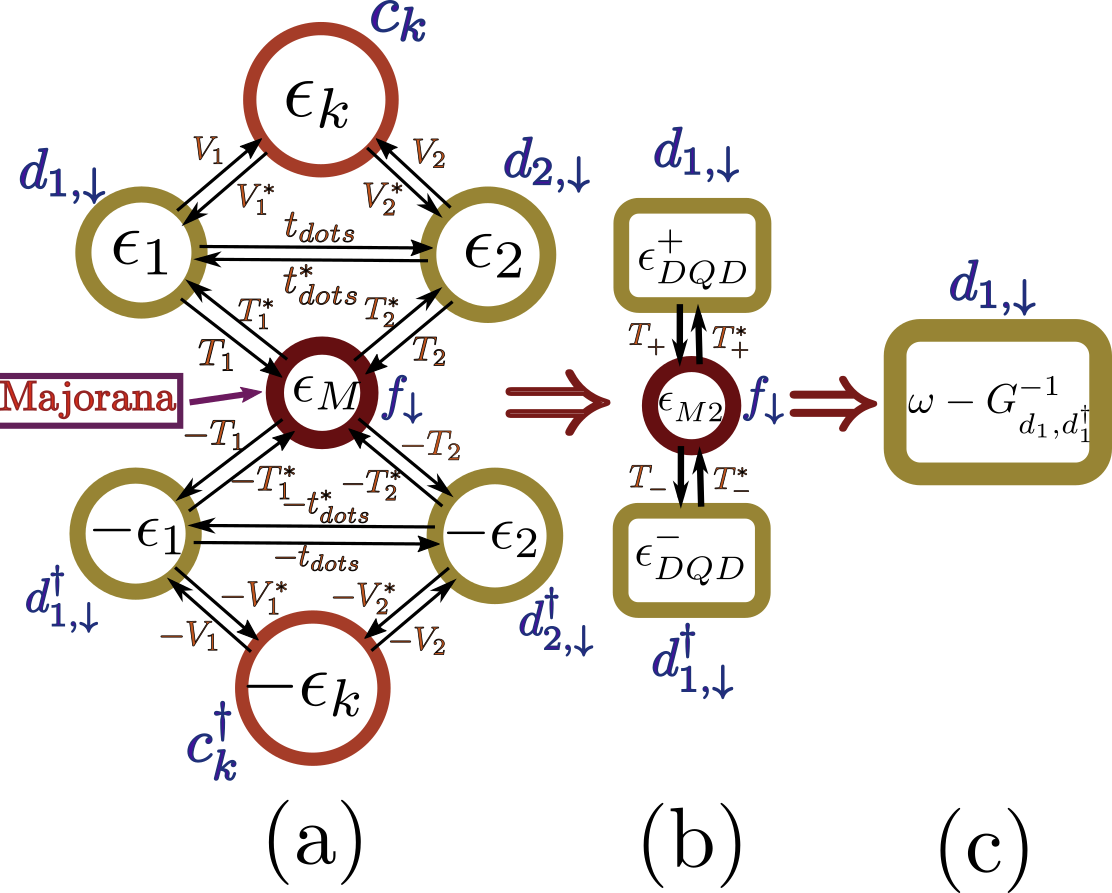
\includegraphics[scale=0.29]{Graficos/Graphs-DQD-M-Pro.png}
    % 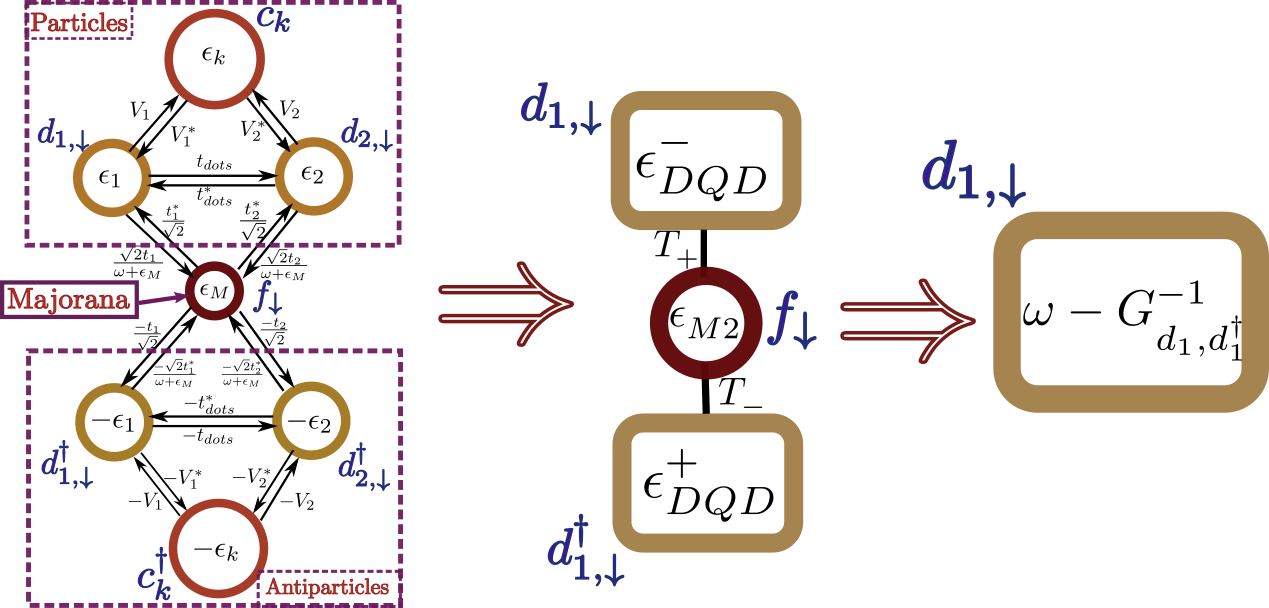
\includegraphics[scale=0.25]{Graficos/graphContractions.png}
    \caption{ Graph-Gauss-Jordan algorithm \cite{spielman_algorithms_2010}  applied to the DQD-Majorana model (a) Initial transport flow diagram  (b) Graph obtained after removing vertexes $c_{k\dw},c^\dagger_{k\dw}, d_{2\dw}$ and $ d^\dagger_{2,\dw}$. New couplings at \eqref{eq:epDQD+-}-\eqref{eq:M2_append} (c) Final graph after removing vertexes $f_\dw, d^\dagger_{1\dw}$. The value of dot $d^\dagger_{1\dw}$ depicts the self energy of the entire system $\omega-G^{-1}_{d_{1\dw},d_{1\dw}^\dagger}$.  \label{fig:GaussJordanGraph}
    }
    %
    
    \end{center}
    \end{figure}

%-----------E N D  F I G U R E  2 ------

The graph associated to  matrix \eqref{eq:TransportMatrix} is in Fig.\ \ref{fig:GaussJordanGraph}. Each vertex depicts the first sub-index of the Green function. The values inside each node are obtained by subtracting the corresponding diagonal term from $\omega$. We usually refer to these terms as ``self-energies" . The couplings are determined by the  off-diagonal terms multiplied by $-1$. 




\subsection{Solution for a DQD attached to a metallic lead}


% %-----------F I G U R E  Graph ------
        \begin{figure}[t]
        \begin{center}
        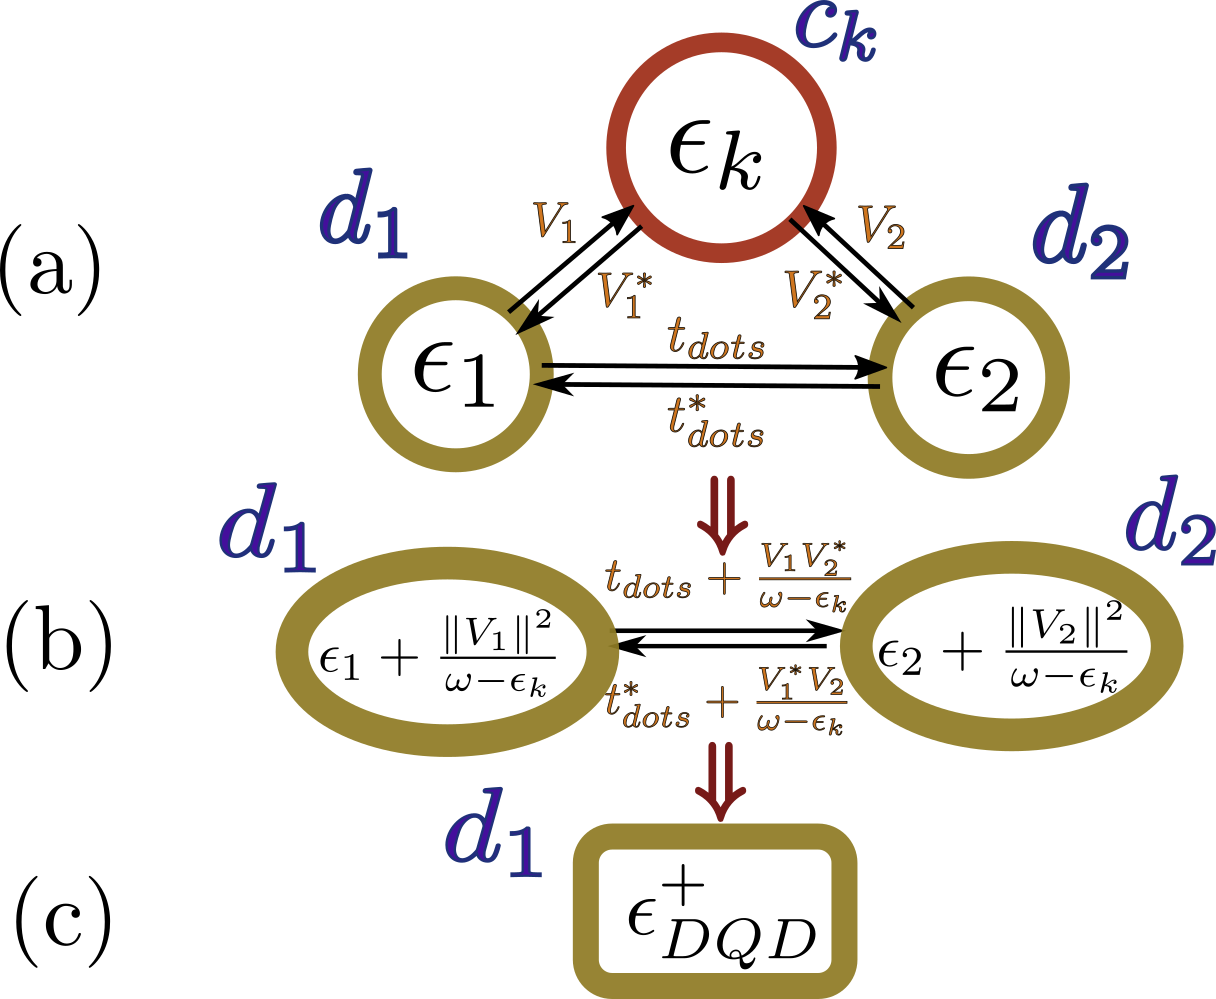
\includegraphics[scale=0.25]{Graficos/Graph_DQD-Pro.png}
        \caption{ Graph-Gauss-Jordan  algorithm applied  to  a DQD attached to a lead. (a) Initial transport flow diagram  (b) Graph obtained after removing vertex $c_{k\dw}$ .  (c) Remaining vertex with self energy $\ep^+_{DQD}$ .
        }
        %
        \label{fig:GraphsDQD}
        \end{center}
        \end{figure}
%-----------E N D  F I G U R E  1 ------




Before attempting to solve the entire system, we will proceed to explain the  Graph-Gauss-Jordan \cite{spielman_algorithms_2010} elimination  process  in a  DQD-model without Majorana fermions $(t_1= t_2=0)$. This is equivalent to find the solution for the $3\times 3$ upper-left block matrix in \eqref{eq:TransportMatrix} 
\begin{equation}
        \left[\begin{array}{ccc}
    \omega-\epsilon_{1} & -V_{1} & -t_{dots}\\
    -V_{1}^{*} & \omega-\epsilon_{k} & -V_{2}\\
    -t_{dots}^{*} & -V_{2}^{*} & \omega-\epsilon_{2}
    \end{array}\right], \label{eq:DQDMatrix}
\end{equation}

\noindent which can be represented by the graph FIG.\ref{fig:GraphsDQD}(a). To eliminate the vertex $c_{k\dw}$ we just need to subtract from \eqref{eq:DQDMatrix} the rank-$1$ matrix that cancels the row and the column corresponding to $c_{k\dw}$. This matrix is 
\begin{equation}
        \left[\begin{array}{ccc}
    \frac{V_{1}^{*}V_{1}}{\omega-\epsilon_{k}} & -V_{1}^{*} & \frac{V_{2}V_{1}^{*}}{\omega-\epsilon_{k}}\\
    -V_{1} & \omega-\epsilon_{k} & -V_{2}\\
    \frac{V_{2}^{*}V_{1}}{\omega-\epsilon_{k}} & -V_{2}^{*} & \frac{V_{2}^{*}V_{2}}{\omega-\epsilon_{k}}
    \end{array}\right]. \label{eq:rank1}
\end{equation}
The result of \eqref{eq:DQDMatrix} -  \eqref{eq:rank1} is 

\begin{equation}
        \left[\begin{array}{ccc}
    \omega-\epsilon_{1}-\frac{V_{1}^{*}V_{1}}{\omega-\epsilon_{k}} & 0 & -t_{dots}-\frac{V_{2}V_{1}^{*}}{\omega-\epsilon_{k}}\\
    0 & 0 & 0\\
    -t_{dots}^{*}-\frac{V_{2}^{*}V_{1}}{\omega-\epsilon_{k}} & 0 & \omega-\epsilon_{2}-\frac{V_{2}V_{1}^{*}}{\omega-\epsilon_{k}}
    \end{array}\right]
\end{equation}
\noindent which is mapped to the graph in Fig.\ \ref{fig:GraphsDQD}(b).

Note that it is possible to associate the correction to the energies and couplings in Fig.\ \ref{fig:GraphsDQD}(b) to the walks passing through the vertex $c_{k\dw}$.  For instance, $d_{1\dw}$'s energy $\epsilon_1$ gets an extra-term $\frac{V_{1}^{*}V_{1}}{\omega-\epsilon_{k}}$ representing an additional walk  from $d_{1\dw}$ to $d_{1\dw}$ passing through  $c_{k\dw}$. The terms $V_1^*$ and $V_1$ represent a movement from $d_{1\dw}$ to $c_{k\dw}$ and vice versa, while the division by $\omega-\epsilon_{k}$ can be thought as a penalty for  passing through $c_{k\dw}$.  The same logic applies to the  coupling terms. The correction to $t_{dots}$ is $\frac{V_{1}^{*}V_{2}}{\omega-\epsilon_{k}}$ which corresponds to a path from $d_{1\dw}$ to $d_{2\dw}$ passing through the removed vertex $c_{k\dw}$. Note that this term includes the multiplication of both couplings with the vertex divided by $\omega-\epsilon_k$. This correspondence between the energy correction and eliminated paths through the graph makes this process straightforward. 


The next step is to remove the vertex $d_{2\dw}$ following the same procedure. At the end, the "self-energy" inside  vertex $d_{1\dw}$ will be
\begin{equation}
    \epsilon^+_{DQD}=\epsilon_{1}+\sum_{\mathbf{k}}\frac{V_{1}V_{1}^{*}}{\omega-\epsilon_{\mathbf{k}}}+\frac{\left\Vert t_{dots}+\sum_{\mathbf{k}}\frac{V_{1}V_{2}^{*}}{\omega-\epsilon_{\mathbf{k}}}\right\Vert ^{2}}{\omega-\epsilon_{2}-\sum_{\mathbf{k}}\frac{V_{2}V_{2}^{*}}{\omega-\epsilon_{\mathbf{k}}}} \label{eq:EnDQD}
\end{equation}
and the green function of $\Green{d_{1\dw}d^\dagger_{1\dw}}$ in a DQD is $\frac{1}{\omega -  \epsilon^+_{DQD}}$ (see Fig.\ \ref{fig:GraphsDQD}(c)).

\subsection{The Graph-Gauss-Jordan algorithm}

The previous method to compute the Green function  $\Green{d,d^\dagger}$ of an operator $d$ can be summarized in the following steps:

\begin{enumerate}
    \item Computing the equations of motion with the second term of the Green function fixed in the creation operator $d^\dagger$. 
     \item  Mapping the linear system to the associated directed flow graph. The self-energy of each vertex $\nu_n$ is taken as $\omega-\epsilon_{n}$.  The coupling terms $t_{ij}$ connecting vertexes $\nu_i$ to $\nu_j$ are given by the the $(i,j)$-off-diagonal terms of the matrix multiplied by $-1$. Set $\nu_1 = d$.  
    \item Removing one-by-one the vertexes of the graph, starting by the last vertex $\nu_N$. When a  vertex $\nu_n$ is removed, the extra-terms of the energies and couplings are computed as follows:
      \begin{enumerate}
        \item Energies: Let $t_{in}$,\ $t_{ni}$ be the coupling constants associated to the edges from $\nu_i$ to $\nu_n$  and from $\nu_n$ to $\nu_i$ respectively. Note that $t_{ni} = t_{in}^*$ since the matrix $\mathcal{T}$ is hermitian. Then there is an indirect path from $\nu_i$ to itself passing through $\nu_n$. When  $\nu_n$ is eliminated , the extra-term added to $\epsilon_{i}$ is   $\frac{t_{in}t^*_{in}}{\omega-\epsilon_{n}}$. 
        \item Couplings: Let $t_{in},\ t_{nj}$ be the coupling constants associated to the edges from $\nu_i$ to $\nu_n$  and from $\nu_n$ to $\nu_j$. Then there is an indirect path from $\nu_i$ to $\nu_j$ passing through $\nu_n$. When  $\nu_n$ is eliminated , the extra-term added to $t_{ij}$ is   $\frac{t_{in}t_{nj}}{\omega-\epsilon_{\nu}}$. 
        \end{enumerate}
    \ignorespacesafterend  
    This process is iterated from $n=N$ till $n=1$.
    \item The self-energy in the remaining vertex $\nu_1 = d$ is related with the green-function as $\epsilon_d = \omega -\frac{1}{ \Green{d,d^\dagger}}$.
\end{enumerate}
    
 
   
    % Computing the extra-terms of the energies and couplings associated to the walks passing through the removed vertex as follows: \\  Let $\epsilon_\nu$ be the self energy of $\nu$. For each two vertexes $\nu_1$ and $\nu_2$ coupled to $\nu$, let $c_1$,$c_2$ be the respective coupling constants. Then the extra-term associated to the direct coupling of $\nu_1$ and $\nu_2$ is $\frac{c_{1}c_{2}}{\omega-\epsilon_{\nu}}$. 
        

The previous algorithm is equivalent to the Gauss-Jordan elimination process with two additional insights: 1) It has linear order. 2) The graph structure allows to identify minimal and maximal cutting points which simplifies the complexity of the solution. As pointed out in previous sources \cite{spielman_algorithms_2010}, selecting a good order of elimination of the vertexes can improve the efficiency of the algorithm. In FIG. \ref{fig:GaussJordanGraph}.(a), for instance, it is better to start eliminating the vertexes at the edges, $c_{k\dw}$ and $c_{k\dw}^\dagger$, each one is coupled to just two nodes. Instead, the Majorana operator $f_\dw$ will be eliminated at last since it is the one with higher number of couplings.  
\subsection{Solution for a DQD-Majorana system}
From these ideas, we can execute the graph elimination process on the model in FIG. \ref{fig:GaussJordanGraph}(a) .  We start by removing the vertexes $c_{k\dw},c^\dagger_k, d_{2,\dw}$ and $ d^\dagger_{2,\dw}$, in that order (See Fig.\ \ref{fig:GaussJordanGraph}(b)). The energies associated to $d_{1,\dw}$ and $d^\dagger_{1,\dw}$ will be similar to \eqref{eq:EnDQD} obtaining
\begin{equation}
    \epsilon_{DQD}^{\pm}=\pm\epsilon_{1}+\sum_{\mathbf{k}}\frac{V_{1}V_{1}^{*}}{\omega-\epsilon_{\mathbf{k}}}+\frac{\left\Vert \pm t_{dots}+\sum_{\mathbf{k}}\frac{V_{1}V_{2}^{*}}{\omega-\epsilon_{\mathbf{k}}}\right\Vert ^{2}}{\omega\mp\epsilon_{2}-\sum_{\mathbf{k}}\frac{V_{2}V_{2}^{*}}{\omega-\epsilon_{\mathbf{k}}}} \; \label{eq:epDQD+-}
\end{equation}
\noindent There is also a correction in the couplings between the Majorana mode and $d_{1,\dw}$, $d^\dagger_{1,\dw}$ given by 
\begin{equation}
    T_{\pm}=\pm t_{1}\pm t_{2}\frac{\left(\pm t_{dots}+\sum_{\mathbf{k}}\frac{V_{1}V_{2}^{*}}{\omega-\epsilon_{\mathbf{k}}}\right)}{\omega\mp\epsilon_{2}-\sum_{\mathbf{k}}\frac{V_{2}V_{2}^{*}}{\omega-\epsilon_{\mathbf{k}}}}. \label{eq:T+-}
\end{equation}
In addition there appears a self-energyb $\epsilon_M$ in the  Majorana operator due to the coupling between $f_\dw$ and $d_{2\dw}$. This new term is 
\begin{equation}
    \begin{aligned}
        \epsilon_{M}=  \omega -\frac{\left\Vert t_{2}\right\Vert ^{2} } {\omega-\epsilon_{2}-\sum_{\mathbf{k}}\frac{V_{2}V_{2}^{*}}{\omega-\epsilon_{\mathbf{k}}}} 
         - \frac{\left\Vert t_{2}\right\Vert ^{2}}{\omega+\epsilon_{2}-\sum_{\mathbf{k}}\frac{V_{2}V_{2}^{*}}{\omega+\epsilon_{\mathbf{k}}}}. 
    \end{aligned}
    \label{eq:M2_append}
\end{equation}
With all the terms of the graph in Fig.\ \ref{fig:GaussJordanGraph}.(b) computed, it only remains to remove the vertexes $d^\dagger_{1\dw}$ and $f_\dw$, in that order. This will lead us to the final result \eqref{eq:Green_NonInteracting}. 
\begin{equation}
    G_{{d_{1\downarrow},d_{1\downarrow}^{\dagger}}}\left(\omega\right)=\frac{1}{\omega-\epsilon_{DQD}^{+}-\frac{\left\Vert T_{+}\right\Vert ^{2}}{\omega-\epsilon_{M}-\frac{\left\Vert T_{-}\right\Vert ^{2}}{\omega - \epsilon_{DQD}^{-}}}}.
     \label{eq:2Green_NonInteracting}
\end{equation}
\noindent From this analytic expression we can compute rapidly dynamic quantities such as the density of states in the non-interacting regime. In this project, it allowed us to achieve a better understanding of the system in the different couplings, and also, to predict parameters that exhibit an interesting behavior. These parameters where simulated afterwards through NRG, which has a larger run-time. 

We introduced the Graph-Gauss-Jordan algorithm as a simple, didactic and graphical method to solve the equations of motion of quadratic Hamiltonians. We hope for its extended use in condensed matter physics.



%\bibliographystyle{unsrtnat}
%\addcontentsline{toc}{section}{\textbf{References}}
%\bibliography{Majorana_DQD.bib}
\bibliography{Majorana_DQD}





\end{document}

